% Imported from LaTeX_and_pdfs/DGDT_dump.tex; see provenance.json.
\part{Manifolds}


Schuller (2015) \cite{dgdt:Schu2015}

\begin{enumerate}
	\item (strikethrough)
	\item 
	\item transitivity
	\item totality: $a\leq b$ or $b\leq a$, \, $\forall a, b$
\end{enumerate}

\begin{definition}[upper bound]

Schuller, original, version 1: \\
$u \in P$ \textbf{upper bound} to a subset $T\subseteq P$ if \\
$\forall t \in T$ : $t\leq u$ (EY: in $t\leq u$, $\leq$ is for partial ordered set) \\

version 2, possible alternative (bottomline: not right): \\
(of is it $u\in P$ \textbf{upper bound} to a subset $T \subseteq P$ if $\nexists \, t\in T$ s.t. $u\leq t$)

\end{definition}

\section{Examples}

\subsection{Euclidean space}

\subsubsection{$\mathbb{R}^2$}

Consider $\mathbb{R}^2$ as a smooth manifold.  

Clearly, $\mathbb{R}^2$ is covered by 1 chart, with so-called \emph{Cartesian} coordinates (that also happen to be global coordinates, in this particular case): $(\mathbb{R}^2, \mathcal{O}_{\text{std}}, \mathcal{A} = \lbrace = \lbrace (\mathbb{R}^2, \varphi_{\text{cart}} ) \rbrace )$, with the chart (which is a homeomorphism, by definition)
\[
\begin{aligned}
	& \varphi_{\text{cart}} : \mathbb{R}^2 \to \mathbb{R}^2 \\ 
	& \varphi_{\text{cart}} : p \equiv (x,y) \mapsto (x,y)
\end{aligned}
\]
Clearly, $\varphi_{\text{cart}} = 1_{\mathbb{R}^2}$ is a homeomorphism; in fact, it's a smooth diffeomorphism.  

$\mathcal{O}_{\text{std}}$ denotes the so-called ``standard'' topology, that open sets consists of Euclidean $d$-balls.  I will assume this topology for this discussion of $\mathbb{R}^d$'s.  

Clearly, the above discussion generalizes to $\mathbb{R}^d$.  

Consider the so-called \emph{polar} coordinates 
\begin{equation}\label{dgdt:Eq:R2polarcoordinates}
	\begin{aligned}
		& x = r\cos{\varphi} \\ 
		& y = r\sin{\varphi}
	\end{aligned}
\end{equation}
where $r\geq 0$ and $\varphi \in \mathbb{R}$.  

Recall the definition of a coordinate char: a \emph{coordinate chart} (or just chart) on $M$ is a pair $(U, \varphi)$ where $U$ is an open subset of $M$, homeomorphism $\varphi : U \to \widehat{U}$, where open subset $\widehat{U} = \varphi(U) \subseteq \mathbb{R}^n$.

We want to construct a homeomorphism $\varphi^{-1}_{\text{pol}}$ from an open subset $V \subseteq \mathbb{R}^2$ to $M = \mathbb{R}^2$ according to these polar coordinates:
\[
\begin{aligned}
	& \varphi_{\text{pol}}^{-1}: V \subseteq \mathbb{R}^2 \to \varphi_{\text{pol}}^{-1}(V) \subseteq M = \mathbb{R}^2 \\ 
	& \varphi^{-1}_{\text{pol}}:(r,\varphi) \mapsto (x,y)
\end{aligned}
\]
Immediately, from this choice of polar coordinates, we see problems with defining a homeomorphism, which is a bijection by definition.  For instance, let $(\varphi_{\text{pol}}^{-1})^{-1} \equiv \varphi_{\text{pol}}$ (defining this highly suggestive notation), and so 
\[
\begin{aligned}
	& \varphi_{\text{pol}}:\mathbb{R}^2 \to \mathbb{R}^2 \\ 
	& \varphi_{\text{pol}}:(x,y) \mapsto (r,\varphi)
\end{aligned}
\]
The single point, the origin of $\mathbb{R}^2$, gets mapped to many possible values! In other words,
\[
\varphi_{\text{pol}}(0,0) = \lbrace (r,\varphi) | r=0 \text{ and } \varphi \in \mathbb{R} \rbrace
\]
Clearly this must be the case for any kind of coordinates involving $\cos$'s, $\sin$'s, etc. (i.e. transcendental functions).  So the choice of these kinds of coordinates necessitate giving up on the possibility of a single chart covering the entire manifold of the Euclidean space.  

Consider 
\[
\begin{aligned}
	& V := \lbrace (r,\varphi) | r>0, \varphi \in (0,2\pi) \rbrace \subset \mathbb{R}^2 \\ 
	& [0,\infty) \times [0,2\pi ) - V = \lbrace (r,\varphi) | r = 0 \text{ or } \varphi = 0 \rbrace
\end{aligned}
\]
Now $\varphi_{\text{pol}}^{-1}( [0,\infty) \times [0,2\pi)) = \mathbb{R}^2$, i.e. $\varphi_{\text{pol}}^{-1}$ maps $[0,\infty) \times [0,2\pi)$ \emph{onto} $\mathbb{R}^2$. But it maps $\varphi^{-1}_{\text{pol}}(0, \varphi)$ onto $(0, 0)$ for infinitely many values of $\varphi \in [0, 2\pi)$.

Now consider if $\varphi=0$.  Then $\begin{aligned} & \quad \\
	& x = r \\ 
	& y = 0 \end{aligned}$ for $r>0$.  So $x>0$ and $y=0$.  If $r=0$, then $(x,y)=(0,0)$.  Thus
\[
\varphi_{\text{pol}}^{-1}( [0,\infty) \times [0,2\pi)-V) = \lbrace (x,y) | x\geq 0 \text{ and } y=0 \rbrace
\]
(If you have trouble seeing this, think of the union of the cases when $r=0$ or when $\varphi=0$).  Thus
\[
\varphi^{-1}_{\text{pol}}(V) = \lbrace (x,y) | x<0 \text{ or } y \neq 0 \rbrace
\]

Thus, in summary, we can include this chart into atlas $\mathcal{A}$:

\begin{equation} \label{dgdt:Eq:UR2}
	\begin{gathered}
		(U, \varphi_{\text{pol}}) \in \mathcal{A} \\ 
		\begin{aligned}
			U & = \lbrace (x,y) | x<0 \text{ or } y \neq 0 \rbrace  \\
			\varphi_{\text{pol}}(U) & = \lbrace (r,\varphi) | r >0, \varphi \in (0,2\pi) \rbrace
		\end{aligned} \quad \quad \, \begin{aligned}
			& \varphi_{\text{pol}}:U \to \mathbb{R}^2 \\ 
			& \varphi_{\text{pol}}(x,y) = ( \sqrt{x^2 + y^2}, \begin{cases} \text{arccot}{ \left( \frac{x}{y} \right) }  & \text{ if } (x > 0 \text{ and } y \geq 0 ) \text{ or } (x > 0 \text{ and } y \leq 0) \\ \text{arccot}{ \left( \frac{x}{y} \right) } + \pi & \text{ if } ( x < 0 \text{and } y \leq 0) \text{ or } (x \geq 0 \text{ and } y < 0) \end{cases} ) \\ 
			& \varphi^{-1}_{\text{pol}}: \varphi_{\text{pol}}(U) \to \mathbb{R}^2 \\ 
			& \varphi^{-1}_{\text{pol}}(r,\varphi) = (r\cos{\varphi}, r\sin{\varphi}) = (x,y)
		\end{aligned}
	\end{gathered}
\end{equation}
where $0 < \text{arccot}(x) < \pi$, with limits $\lim_{x \to -\infty} \text{arccot}(x) = \pi$ and $\lim_{x \to \infty} \text{arccot}(x) = 0$ being well defined.

Recall the plots of $\arctan$ and $\text{arccot}$:


	
	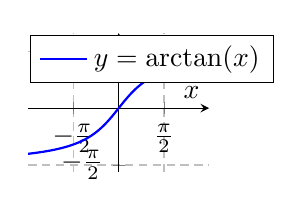
\begin{tikzpicture}
		\begin{axis}[axis lines=middle,xlabel={$x$},ylabel={$y$},
			width=0.32\textwidth,
			trig format plots=rad,
			samples=101,
			unbounded coords=jump,
			xmin=-pi,xmax=pi,
			ymin=-pi/2-0.2,ymax=pi/2+0.5,
			xtick={-pi/2,pi/2},xticklabels={$-\frac{\pi}{2}$,$\frac{\pi}{2}$},
			ytick={-pi/2,pi/2},yticklabels={$-\frac{\pi}{2}$,$\frac{\pi}{2}$},
			grid=major,grid style={densely dashed},
			legend style={at={(0.01,0.99)},anchor=north west}
			]
			\addplot[blue,thick,variable=\t,domain=-pi/2+0.1:pi/2-0.1] ({tan(\t)},\t);
			\addlegendentry{$y=\arctan(x)$}
		\end{axis}
	\end{tikzpicture}

	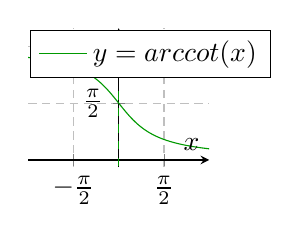
\begin{tikzpicture}
	\begin{axis}[axis lines=middle,xlabel={$x$},ylabel={$y$},
		width=0.32\textwidth,
		trig format plots=rad,
		samples=101,
		unbounded coords=jump,
		xmin=-pi,xmax=pi,
		ymin=-0.0-0.2,ymax=pi+0.5,
		xtick={-pi/2,pi/2},xticklabels={$-\frac{\pi}{2}$,$\frac{\pi}{2}$},
		ytick={0.0, pi/2, pi},yticklabels={$0.0$,$\frac{\pi}{2}$, $\pi$},
		grid=major,grid style={densely dashed},
		legend style={at={(0.01,0.99)},anchor=north west}
		]
		\addplot[green!60!black,variable=\t,domain=-0.0+0.1:pi-0.1] ({cot(\t)},\t);
		\draw[green!60!black,dashed] (0,-2) -- (0,2);
		\addlegendentry{$y=\text{arccot}(x)$}
	\end{axis}
\end{tikzpicture}
	




Let's try to cover $\mathbb{R}^2$ as much as possible with these "polar coordinate"-type charts. Unfortunately, we'll find out that we can't cover the origin in a well-defined (meaning with one-to-one functions) manner, so we'll have to consider $\mathbb{R}^2\backslash 0 := \mathbb{R}^2 - \lbrace 0 \rbrace$ (the Euclidean space $\mathbb{R}^2$ but without the origin).

Repeat some of the steps we did above. Consider open subset 
\[
U_+ = \lbrace (x, y) | x > 0 \text{ or } y \neq 0 \rbrace
\]
obtained by considering
\[
\begin{aligned}
& V_+ = \lbrace (r, \varphi) | r >0, \, \varphi \in (-\pi, \pi) \rbrace \in \mathbb{R}^2 \\
& [0, \infty) \times (-\pi, \pi] - V_+ = \lbrace (r, \varphi) | r = 0 \text{ or } \varphi = \pi \rbrace
\end{aligned}
\]
Consider if $\varphi = \pi$. Then $\begin{aligned} & \quad \\
	& x = -r \\
	& y = 0 \end{aligned}$ \, for $r> 0$, so $x<0 $ and $y=0$. If $r=0$, then $(x, y) = (0,0)$. So $\varphi^{-1}_{\text{pol}, +}(V_+) = \lbrace ( x, y) | x > 0 \text{ or } y\neq 0 \rbrace$

\begin{equation} \label{dgdt:Eq:UR22}
	\begin{gathered}
		(U_+, \varphi_{\text{pol},+}) \in \mathcal{A} \\ 
		\begin{aligned}
			U_+ & = \lbrace (x,y) | x>0 \text{ or } y \neq 0 \rbrace  \\
			\varphi_{\text{pol}, +}(U) & = \lbrace (r,\varphi) | r >0, \varphi \in (-\pi,\pi) \rbrace
		\end{aligned} \\
	 \begin{aligned}
			& \varphi_{\text{pol},+}:U_+ \to \mathbb{R}^2 \backslash 0 \\ 
			& \varphi_{\text{pol},+}(x,y) = ( \sqrt{x^2 + y^2}, \begin{cases} \arctan{ \left( \frac{y}{x} \right) }  & \text{ if } (x > 0 \text{ and } y \geq 0 ) \text{ or } (x > 0 \text{ and } y \leq 0) \\ \arctan{ \left( \frac{y}{x} \right) } + \pi & \text{ if } ( x \leq 0 \text{ and } y > 0)) \\
			\arctan{ \left( \frac{y}{x} \right) } - \pi & \text{ if } (x\leq 0 \text{ and } y < 0) \end{cases} ) \\ 
			& \varphi^{-1}_{\text{pol},+}: \varphi_{\text{pol},+}(U) \to \mathbb{R}^2\backslash 0 \\ 
			& \varphi^{-1}_{\text{pol},+}(r,\varphi) = (r\cos{\varphi}, r\sin{\varphi}) = (x,y)
		\end{aligned}
	\end{gathered}
\end{equation}
where $\pi/ 2 < \arctan(x) < \pi/ 2$, with limits $\lim_{x \to -\infty} \arctan(x) = -\pi/2$ and $\lim_{x \to \infty} \arctan(x) = \pi/2$ being well defined.



\subsection{Spheres}

cf. Example 1.4 (Spheres), Lee (2012) \cite{dgdt:JLee2012}, pp. 5

$\forall \, n \geq 0, \, n \in \mathbb{Z}$, $n$-sphere $\mathbb{S}^n$ is Hausdorff and second-countable because it's topological subspace of $\mathbb{R}^{n+1}$. \\
$\forall \, i = 1, \dots n +1$, let $U_i^+ = \lbrace (x^1, \dots x^{n+1}) \in \mathbb{R}^{n+1}: x^i > 0 \rbrace$. \\
Similarly, let $U_i^- = \lbrace (x^1, \dots x^{n+1})  \in \mathbb{R}^{n+1} : x^i < 0 \rbrace$  \\

Let $f: \mathbb{B}^n \to \mathbb{R}$ be $f(u) = \sqrt{ 1 - |u|^2}$. \\

$\forall \, i =1 , \dots n +1$, $U_i^+ \cap \mathbb{S}^n$ is graph of function
\[
x^i = f(x^1 \dots \widehat{x}^i \dots x^{n+1})
\]

where $\widehat{x}^i$ indicates $x^i$ is omitted, \\
since
\[
\sqrt{ (x^1)^2  + (x^{n+1})^2 } = 1^2 \text{ or } (x^i)^2 = 1 - \sum_{ \substack{ j\neq i \\ i =1} }^{n+1} (x^j)^2 \Longrightarrow x^i = f(x^1, \dots \widehat{x}^i, \dots x^{n+1})
\]

Similarly, $U_i^i \cap \mathbb{S}^n$ is graph of 
\[
x^i = -f(x^1 \dots \widehat{x}^i \dots x^{n+1})
\]
sicne $x^i < 0$.

Thus, $\forall \,$ subset $U_i^{\pm} \cap \mathbb{S}^n$ is locally Eucliean of dim. $n$ nad maps
\[
\begin{aligned}
	& \varphi_i^{\pm} : U_i^{\pm} \cap \mathbb{S}^n \to \mathbb{B}^n \\
	& \varphi_i^{\pm} (x^1 \dots x^{n+1}) = (x^1 \dots \widehat{x}^i \dots x^{n+1})
\end{aligned}
\]
are graph coordinates for $\mathbb{S}^n$.

Since $\forall \,$ pt. $\in \mathbb{S}^n$ is in domain of at least 1 of these $2n+2$ charts, $\mathbb{S}^n$ is a topological $n$-manifold.

cf. Example 1.31 (Spheres), Lee (2012) \cite{dgdt:JLee2012}, pp. 20, \\

$\forall \, i = 1 \dots n+1$, let $(U_i^{\pm}, \varphi_i^{\pm})$ denote graph coordinate charts, s.t.

\[
\begin{aligned}
	& U_i^{\pm} = \lbrace (x^1 \dots x^{n+1}) \in \mathbb{R}^{n+1} : x^i \gtrless 0 \rbrace \\ 
	& \varphi_i^{\pm} : U_i^{\pm} \cap \mathbb{S}^n \to \mathbb{B}^n \\ 
	& \varphi_i^{\pm} (x^1 \dots x^{n+1}) = (x^1, \dots \widehat{x}^i \dots x^{n+1})
\end{aligned}\]

$\forall \, $ distinct $i,j$, transition map $\varphi_i^{\pm} \circ (\varphi_j^{\pm})^{-1}$ is computed; for $i<j$,
\[
\varphi_i^{\pm} \circ (\varphi_j^{\pm})^{-1} (u^1 \dots u^n) = (u^1, \dots \widehat{u}^i \dots \pm \sqrt{1 - |u|^2}, \dots u^n )
\]

with $\sqrt{1- |u|^2}$ in $j$th position; similarly for $i =j$. \\

Also $\varphi_i^+ \circ (\varphi_i^-)^{-1} (x^1, \dots x^n) = \varphi_i^{+} (x^1 \dots - \sqrt{1 - \sum_i(x^i)^2} \dots x^n) = (x^1 \dots x^n)$. \\

So $\varphi_i^+ \circ (\varphi_i)^{-1} = \varphi_i^- \circ (\varphi_i^+)^{-1} = 1_{\mathbb{B}^n}$. \\

$\lbrace (U_i^{\pm}, \varphi_i^{\pm}) \rbrace$ is a smooth atlas, defines smooth structure on $\mathbb{S}^n$. This is its \textbf{standard smooth structure}.


\problemhead{1, Wald (1984) \cite{dgdt:Wald1984}}
\begin{enumerate}
	\item[(a)] In Wald's notation, $f^+_i : O_i^+ \to D$; compare Lee's notation against Wald's, respectively:
	
	\[
	\varphi_i^{\pm} : U^{\pm}_i \cap S^n \to \mathbb{B}^n \equiv f_i^{\pm} : O_i^{\pm} \to D^n
	\]
	
	\[
	\varphi_i^{\pm} \circ (\varphi_j^{\pm})^{-1} (x^1 \dots x^n) = \varphi_i^{\pm}( x^1, \dots \pm \sqrt{ 1 -\sum_{k=1}^n (x^k)^2} \dots x^n) = (x^1 \dots \widehat{x}^i \dots \pm \sqrt{ 1 - \sum_{k=1}^n (x^k)^2 } , \dots x^n)
	\]
Clearly, $\varphi_i^{\pm} \circ (\varphi_j^{\pm})^{-1}$ is $C^{\infty}$ by taking $\frac{ \partial}{\partial x^k} $ to any order, since $\mathbb{B}^n$ doesn't include its boundary.

	\item[(b)] See \emph{stereographic projection}: 

	\textbf{north pole} $N = (0, \dots 0, 1) \in S^n \subseteq \mathbb{R}^{n+1}$ \\
\textbf{south pole} $S = (0, \dots 0,-1) \in S^n \subseteq \mathbb{R}^{n+1}$ \\
\textbf{stereographic projection} 
\[
\begin{aligned}
	& \sigma : \mathbb{S}^n \setminus \lbrace N \rbrace \to \mathbb{R}^n \\
	& \sigma(x^1 , \dots x^{n+1}) = \frac{ (x^1, \dots x^n ) }{ 1 - x^{n+1}} 
\end{aligned}
\]
\[
\begin{aligned}
	& \widetilde{\sigma}: \mathbb{S}^n \setminus \lbrace S \rbrace \to \mathbb{R}^n \\
	& \widetilde{\sigma}(x^1 , \dots x^{n+1}) = -\sigma(-x) = \frac{ x^1, \dots x^n }{ 1 + x^{n+1}}
\end{aligned}
\]

\end{enumerate}

\problemhead{1-7, Lee (2012) \cite{dgdt:JLee2012}, \textbf{Stereographic projection of spheres}}

Let $N$ denote the \textbf{north pole} $(0, \dots, 0, 1) \in \mathbb{S}^n \subseteq \mathbb{R}^{n+1}$, and let S denote the \textbf{south pole} $(0, \dots , 0 , -1)$. Define the \textbf{stereographic projection} $\sigma: \mathbb{S}^n \setminus \lbrace N \rbrace \to \mathbb{R}^n$ by 
\[
\sigma(x^1, \dots x^{n+1}) = \frac{ (x^1, \dots x^n ) }{ 1 - x^{n+1}}
\]
Let $\widetilde{\sigma}(x) = -\sigma(-x)$ for $x\in \mathbb{S}^n \setminus \lbrace S \rbrace$.

\begin{enumerate}
	\item[(a)] So given a \\
	\textbf{north pole} $N = (0, \dots 0, 1) \in S^n \subseteq \mathbb{R}^{n+1}$ \\
	\textbf{south pole} $S = (0, \dots 0,-1) \in S^n \subseteq \mathbb{R}^{n+1}$ \\
	\textbf{stereographic projection} 
	\[
	\begin{aligned}
		& \sigma : \mathbb{S}^n \setminus \lbrace N \rbrace \to \mathbb{R}^n \\
		& \sigma(x^1 , \dots x^{n+1}) = \frac{ (x^1, \dots x^n ) }{ 1 - x^{n+1}} 
	\end{aligned}
	\]
	\[
	\begin{aligned}
		& \widetilde{\sigma}: \mathbb{S}^n \setminus \lbrace S \rbrace \to \mathbb{R}^n \\
		& \widetilde{\sigma}(x^1 , \dots x^{n+1}) = -\sigma(-x) = \frac{ x^1, \dots x^n }{ 1 + x^{n+1}}
	\end{aligned}
	\]

Consider $\mathbf{x} \in \mathbb{S}^n \setminus \lbrace N \rbrace \to \mathbb{R}^n$, $\mathbf{x} = (x^1 \dots x^{n+1})$.
\[
\begin{gathered}
	N + t(\mathbf{x} - N) = \mathbf{x}' \Longrightarrow 1 + t(x^{n+1} - 1 ) = 0 \text{ or } t = \frac{1}{ 1- x^{n+1}} \\
	(x')^i = \frac{x^i}{ 1 - x^{n+1}}  \quad \, \forall \, i \neq n + 1
\Longrightarrow \sigma(x^1 \dots x^{n+1}) = \frac{ (x^1, \dots x^n) }{ 1 - x^{n+1}}
\end{gathered}
\]
Thus we have a stereographic projection from the north pole.

\[
\begin{gathered}
	S + t(\mathbf{x} - S) = \mathbf{x}' \Longrightarrow 1 + t(x^{n+1} + 1) = 0 \text{ or } t= \frac{1}{1 + x^{n+1}} \\
	(x')^i = \frac{x^i }{ 1 + x^{n+1}} \quad \, \forall \, i \neq n + 1 \\
	\Longrightarrow \widetilde{\sigma}(x^1 \dots x^{n+1}) = \frac{ (x^1, \dots x^n) }{ 1 + x^{n+1}}
\end{gathered}
\]
\textbf{Thus we have a stereographic projection from the south pole}.

\item[b]
\[
\begin{gathered}
\begin{aligned}
	& \sigma^{-1} (u^1 \dots u^n) = \frac{(2u^1 \dots 2u^n, |u|^2 - 1) }{ |u|^2 + 1 } \\
	& \sigma \circ \sigma^{-1}(u^1 \dots u^n) = \frac{ (2u^1 \dots 2u^n) }{ |u|^2 + 1 } / \left( 1 - \frac{ |u|^2 - 1 }{ |u|^2 + 1 } \right) = (u^1, \dots u^n)
\end{aligned}	\\
\sigma^{-1} \circ \sigma(x^1, \dots x^{n+1}) = \sigma^{-1} \frac{ (x^1 \dots x^n) }{ 1 - x^{n+1} } = \frac{ \left(\frac{ 2 x^1}{ 1 - x^{n+1} } , \dots \frac{2x^n}{1 - x^{n+1} } , \frac{ (x^1)^2 + \dots + (x^n)^2 }{ ( 1- x^{n+1})^2 } - 1 \right) }{ \frac{ (x^1)^2 + \dots + (x^n)^2}{ (1- x^{n+1})^2 } + 1 } = \\
= \frac{ \left( \frac{ 2 x^1}{ 1 - x^{n+1}} \dots \frac{2x^n}{1- x^{n+1}} , \frac{ (x^1)^2 + \dots + (x^n)^2 }{ (1-x^{n+1})^2} - \frac{ 1 - 2x^{n+1} + (x^{n+1})^2 }{ (1- x^{n+1})^2} \right) }{ \frac{2(1-x^{n+1})}{(1-x^{n+1})^2} } = \left( x^1, \dots x^n , \frac{ 1 - (x^{n+1})^2 - 1 + 2x^{n+1} - (x^{n+1})^2 }{ \frac{ 2 }{ 1 - x^{n+1}} (1- x^{n+1})^2 } \right) = \\
= (x^1, \dots x^n , \frac{2 x^{n+1} ( 1 -x^{n+1}) }{ \frac{ 2 }{ 1 - x^{n+1}} ( 1 - x^{n+1})^2 } ) = (x^1, \dots x^{n+1})
\end{gathered}
\]
\item[(c)] Compute the transition map $\widetilde{\sigma} \circ \sigma^{-1}$. (The coordinates defined by $\sigma$ or $\widetilde{\sigma}$ are called \textbf{stereographic coordinates}).

\[
\begin{gathered}
	\widetilde{\sigma} \circ \sigma^{-1}(u^1 \dots u^n) = \widetilde{\sigma} \frac{(2u^1 \dots 2u^n, |u|^2-1) }{ |u|^2 +  1} = \frac{ \frac{2u^1}{ |u|^2 + 1} , \dots \frac{2u^n}{ |u|^2 + 1} }{ 1 + \frac{ |u|^2 - 1 }{ |u|^2 + 1} } = \frac{ \frac{2u^1}{ |u|^2 + 1} , \dots \frac{2u^n}{ |u|^2 + 1} }{  \frac{2|u|^2}{ |u|^2 + 1} } = \\
	= \boxed{ \left( \frac{u^1}{ |u|^2} , \dots , \frac{u^n}{ |u|^2} \right) }
\end{gathered}
\]

\end{enumerate}

\subsubsection{Polar coordinates}

Consider 
\[
\mathbf{x}(\theta, \varphi) = (s\theta c\varphi, s\theta s\varphi, c\theta)
\]
\[
\begin{aligned}
& \theta = \arccos{z}, \quad \, \theta \in [0, \pi] , \, z \in [0,1] \\
& \begin{gathered}
\varphi = \begin{cases}
	& \arctan{ \left( \frac{y}{x} \right) } \text{ if } x > 0, \, \varphi \in ( \frac{-\pi}{2}, \frac{\pi}{2}) \\
	& \arctan{ \left( \frac{y}{x} \right) }  + \pi if x < 0 \text{ and } y > 0, \, \varphi \in (\frac{\pi}{2}, \pi) \\
	& \arctan{ \left( \frac{y}{x} \right) }  - \pi if x < 0 \text{ and } y < 0, \, \varphi \in (-\pi, \frac{-\pi}{2}) \\ 
	& \frac{\pi}{2} \text{ if } x = 0, y = 1\\
	& \frac{-\pi}{2} \text{ if } x= 0 , y = -1
\end{cases}	
\end{gathered}
\end{aligned}
\]


\section{Inverse Function Theorem}

Shastri (2011) had a thorough and lucid and explicit explanation of the Inverse Function Theorem \cite{dgdt:AShastri2011}.  I will recap it here.  The following is also a blend of Wienhard's Handout 4 \url{https://web.math.princeton.edu/~wienhard/teaching/M327/handout4.pdf}

\begin{definition}
  Let $(X,a)$ metric space.  

\textbf{contraction} $\phi:X \to X$ if $\exists \, $ constant $0<c<1$ s.t. $\forall \, x,y \in X$
\[
d(\phi(x),\phi(y)) \leq cd(x,y)
\]
\end{definition}

\begin{theorem}[Contraction Mapping Principle]
  Let $(X,d)$ complete metric space.  \\
Then $\forall \, $ contraction $\phi:X\to X$, $\exists \, ! y\in X$ s.t. $\phi(y) = y$, $y$ \emph{fixed pt.}
\end{theorem}

\begin{proof}
  Recall def. of complete metric space $X$, $X$ metric space s.t. $\forall \, $ Cauchy sequence in $X$ is convergent in $X$ (i.e. has limit in $X$).  

$\forall \, x_0 \in X$,
Define $\begin{aligned} & \quad \\
  & x_1 = \phi(x_0) \\ 
  & x_2 = \phi(x_1) \\ 
  & \vdots \\
  & x_j = \phi(x_{j-1}) \\ 
  & \vdots \\
  & x_n = \phi(x_{n-1})
\end{aligned}$

\[
\begin{gathered}
  d(x_{n+1},x_n) = d(\phi(x_n),\phi(x_{n-1})) \leq c d(x_n,x_{n-1}) \leq \dots \leq c^nd(x_1,x_0)
\end{gathered}
\]
for some $0< c<1$.

\[
d(x_m,x_n) \leq d(x_n,x_{n-1}) + d(x_{n-1},x_m) \leq d(x_n,x_{n-1}) + d(x_{n-1},x_{n-2}) + \dots + d(x_{m+1},x_m) \leq \sum_{k=n-1}^m c^k d(x_1,x_0)
\]
Thus, $\forall \, \epsilon >0$, $\exists \, n_0 >0$, ($n_0$ large enough) s.t. $\forall \, m ,n\in \mathbb{N}$ s.t. $n_0 < n <m$, 
\[
d(x_m,x_n) \leq \sum_{k=n-1}^m c^k d(x_1,x_0) < \epsilon d(x_1,x_0)
\]
Thus, $\lbrace x_n \rbrace$ Cauchy sequence.  Since $X$ complete, $\exists \, $ limit pt. $y \in X$ of $\lbrace x_n \rbrace$.  
\[
\phi(y) = \phi(\lim_n x_n) = \lim_n \phi(x_n) = \lim_n x_{n+1} = y
\]
Since by def. of $y$ limit pt. of $\lbrace x_n \rbrace$, $\forall \, \epsilon >0$, then $\lbrace n | |x_n -y|\leq \epsilon, \, n \in \mathbb{N}\rbrace$ is infinite.  

Consider $\delta > \mathbb{N}$.  Consider $\lbrace n | |x_n-y| \leq \delta, n \in \mathbb{N}\rbrace$ 

$\exists \, N_{\delta} \in \mathbb{N}$ s.t. $\forall \, n > N_{\delta}$, $|x_n-y|< \delta$; otherwise, $\forall \, N_{\delta}$, $\exists \, n > N_{\delta}$ s.t. $|x_n - y| \geq \delta$.  Then $\lbrace n | |x_n -y| \leq \delta , n \in \mathbb{N} \rbrace$ finite.  Contradiction.  

$\phi$ cont. so by def. $\forall \, \epsilon >0$, $\exists \, \delta >0$ s.t. if $|x_n -y| < \delta$, then $|\phi(x_n) - \phi(y) | < \epsilon$.  

Pick $N_{\delta}$ s.t. $\forall \, n > N_{\delta}$, $|x_n-y| < \delta$, and so $|\phi(x_n) - \phi(y)|< \epsilon$. There are infinitely many $\phi(x_n)$'s that satisfy this, and so $\phi(y)$ is a limit pt.  

If $\exists \, y_1,y_2 \in X$ s.t. $\begin{aligned} & \quad \\
  & \phi(y_1) = y_1 \\ 
  & \phi(y_2) = y_2 \end{aligned}$, then
\[
d(y_1,y_2) = d(\phi(y_1), \phi(y_2)) \leq c d(y_1,y_2) \text{ with } c <1
\]
so $c=1$
\end{proof}


\begin{theorem}[Inverse Function Theorem]
  Suppose open $U \subset \mathbb{R}^n$, let $C^1 \, f: U \to \mathbb{R}^n$, $x_0 \in U$ s.t. $Df(x_0)$ invertible.  



Then $\exists \,$ open neighborhoods $V\ni x_0$, $W \ni f(x_0)$ s.t. $V\subseteq U$ and $W\subseteq \mathbb{R}^n$, respectively, and s.t.

\begin{enumerate}
\item[(i)] $f: V\to W$ bijection
\item[(ii)] $g = f^{-1}:V \to U$ differentiable, i.e. $g = f^{-1}:W\to V$ is $C^1$
\item[(iii)] $D(f^{-1}) $ cont. on $W$.  
\item[(iv)] $Dg(y) = (Df(g(y)))^{-1}$ \, $\forall \, y \in W$
\end{enumerate}
Also, notice that $f(g(y)) = y \, \forall \, y \in W$.  
\end{theorem}

\begin{proof}


Consider $\widetilde{f}(x) = (Df(x_0))^{-1}(f(x+x_0) - f(x_0))$.  Then \\
\phantom{Consider} $\widetilde{f}(0) = 0$ and 
\[
\begin{aligned}
  &  D\widetilde{f}= (Df(x_0))^{-1}(Df(x+x_0) -0)  \\
  & D\widetilde{f}(0) = (Df(x_0))^{-1}Df(x_0)=1
\end{aligned}
\]  
So let $\widetilde{f}\to f$ (notation) and so assume, without loss of generality, that $U\ni 0$, $f(0)=0$, $Df(0)=1$

Choose $0 < \epsilon \leq \frac{1}{2}$.  Let $0< \delta <1$ s.t. open ball $V = B_{\delta}(0) \subseteq U$, and $\| Df(x)-1\| < \epsilon$.  $\forall \, x \in U$, since $Df$ cont. at $0$.  

Let $W=f(V)$.  

$\forall \, y \in W$, define $\begin{aligned} & \quad \\
  & \phi_y : V \to \mathbb{R}^n \\
  & \phi_y(x) = x + (y-f(x))\end{aligned}$

\[
\begin{aligned}
  & D(\phi_y)(x) = 1 + - Df(x) \quad \, \forall \, x \in V \\ 
  & \| D(\phi_y)(x) \| = \| 1 - Df(x) \| \leq \epsilon <1
\end{aligned}
\]

$\forall \, x_1 ,x_2 \in V$, by mean value Thm. (not the equality that is only valid in 1-dim., but the inequality, that's valid for $\mathbb{R}^d$, 
\[
\| \phi_y(x_1) - \phi_y(x_2) \| \leq \| D(\phi_y)(x') \| \| x_1 - x_2 \| 
\]
for some $x' = cx_2 + (1-c)x_1$, $c\in [0,1]$.  $V$ only needed to be convex set.  
\[
\Longrightarrow \| \phi_y(x_1) - \phi_y(x_2) \| \leq \epsilon \| x_1 - x_2 \|
\]
Then $\phi_y$ contraction mapping.  

Suppose $f(x_1) = f(x_2)=y$, $x_1,x_2 \in V$.  
\[
\begin{gathered}
\begin{aligned}
  & \phi_y(x_1) =x_1 \\ 
  & \phi_y(x_2) =x_2  
\end{aligned} \\
\| \phi_y(x_1) - \phi_y(x_2) \| = \| x_1 - x_2 \| \leq \epsilon \| x_1 - x_2 \| \quad \, \forall \, \epsilon > 0 \Longrightarrow x_1 = x_2 
\end{gathered}
\]
$\Longrightarrow \left. f\right|_U$ injective.

$W=f(V)$, so $f:V\to W$ surjective.  $f$ bijective.  

Fix $y_0 \in W$, $y_0 = f(x_0)$, $x_0 \in V$.  \\
Let $r>0$ s.t. $B_r(x_0) \subset V$.  \\
Consider $B_{r\epsilon}(y_0)$.  If $y\in B_{r\epsilon}(y_0)$.  
\[
\begin{gathered}
  r\epsilon > \| y-y_0 \| = \| y - f(x_0) \| = \| \phi_y(x_0) - x_0 \| \text{ with } \\
  \phi_y(x) = x + (y-f(x))
\end{gathered}
\]

If $x\in B_r(x_0)$, 
\[
\| \phi_y(x) -x_0 \| \leq \| \phi_y(x) - \phi_y(x_0) \|  + \| \phi_y(x_0) - x_0 \| \leq \epsilon \| x-x_0 \| + r\epsilon < 2 r\epsilon = r
\]



Thus $\phi(B_r(x_0)) = B_r(x_0)$.

By contraction mapping principle, $\exists \, a \in B_r(x_0)$, s.t. $\phi_y(a)=a$.  Then $\phi_y(a) = a+ (y-f(a)) = a \Longrightarrow f(a) =y$.  

$y\in f(V) = W$.  

So $B_{r\epsilon}(y_0) \subset W$.  $W$ open.  

Let $\text{Mat}(n,n) \equiv $ space of all $n\times n$ matrices; $\text{Mat}(n,n)  = \mathbb{R}^{n^2}$.  


\end{proof}

There is a proof of the implicit function theorem and its various forms in Shastri (2011) \cite{dgdt:AShastri2011}, but I found Wienhard's Handout 4 for Math 327 to be clearer.\footnote{\url{https://web.math.princeton.edu/~wienhard/teaching/M327/handout4.pdf}}

\begin{theorem}[Implicit Function Theorem]
Let open $U \subset \mathbb{R}^{m+n} \equiv \mathbb{R}^m \times \mathbb{R}^n$  \\
\phantom{Let} $C^1 \, f:U \to \mathbb{R}^n $ \\
\phantom{Let} $(a,b) \in U$ s.t. $f(a,b) = 0$ and $\left. D_y f\right|_{(a,b)}$ invertible.  

Then $\exists \, $ open $V \ni (a,b)$, $V \subset U$ \\
\phantom{Then} $\exists \, $ open neighborhood $W \ni a$, $W \subseteq \mathbb{R}^m$ \\
\phantom{Then} $\exists \, !$ \, $C^1 \, g:W \to \mathbb{R}^n$ s.t.
\[
\lbrace (x,y) \in V | f(x,y) =0 \rbrace = \lbrace (x,g(x)) | x \in W \rbrace
\]
Moreover,
\[
dg_x = - \left. (d_yf)^{-1} \right|_{(x,g(x))} \left. d_x f\right|_{(x,g(x))}
\]
and $g$ smooth if $f$.  
\end{theorem}

\begin{proof}
  Define $\begin{aligned} & \quad \\
    & F: U \to \mathbb{R}^{m+n}   \\
    & F(x,y) = (x,f(x,y)) \end{aligned}$

Then $F(a,b) = (a,0)$ (given), and 
\[
DF = \left[ \begin{matrix} 1 & \\ 
    \frac{ \partial f^i(x,y)}{ \partial x^j} & \frac{ \partial f^i(x,y) }{ \partial y^j } \end{matrix} \right] \equiv \left[ \begin{matrix} 1 & \\
    D_xf & D_yf \end{matrix} \right]
\]
$DF(a,b)$ invertible.  

By inverse function theorem, since $DF(a,b)$ invertible at pt. $(a,b)$, \\
$\exists \, $ open neighborhoods $\begin{aligned} & \quad \\
  & V \ni (a,b) \subseteq \mathbb{R}^m \times \mathbb{R}^n \\
  & \widetilde{W} \ni (a,0) \subseteq \mathbb{R}^m \times \mathbb{R}^n \end{aligned}$ s.t. $F$ diffeomorphism with $F^{-1}: \widetilde{W} \to V$. 

Set $W = \lbrace x \in \mathbb{R}^m | (x,0) \in \widetilde{W}\rbrace$.  Then $\pi_1(\widetilde{W}) =W$ open in $\mathbb{R}^m$.  

Define $g:W\to \mathbb{R}^n$, 
\[
\begin{aligned}
  & g(x) = \pi_2 \circ F^{-1}(x,0) \text{ or } \\ 
  & F^{-1}(x,0) = (h(x),g(x))
\end{aligned}
\]

Now $FF^{-1}(x,0) = (x,0) = (h(x), f(h(x),g(x)) )$ so $h(x)=x \, \forall \, x \in W$, $0 = f(x,g(x))$.  

Then
\[
\lbrace (x,y) \in V | f(x,y) = 0 \rbrace = \lbrace (x,y) \in V | F(x,y) = (x,0) \rbrace = \lbrace (x,g(x)) | x \in W, 0 = f(x,g(x)) \rbrace
\]
Since $\pi$ smooth and $F^{-1}$ is $C^1$, $g$ is $C^1$.  

To reiterate, $f(x,g(x)) =0$ on $W$.

Using chain rule while differentiating $f(x,g(x))=0$, 
\[
\begin{gathered}
\partial_{x^j} f(x,g(x)) = \frac{ \partial f(x,g(x)) }{ \partial x^k} \frac{ \partial x^k}{ \partial x^j}+ \frac{ \partial f(x,g(x))}{ \partial y^k}\frac{ \partial g^k(x)}{\partial x^j} = \left. D_x f \right|_{(x,g(x))} + \left. (D_yf) \right|_{(x,g(x))} \cdot (Dg)_x = 0 \text{ or }  \\
(Dg)_x = -\left. (D_yf) \right|_{x,g(x)} \left. D_xf \right|_{(x,g(x))}
\end{gathered}
\]



\end{proof}

\section{Immersions}

\begin{definition}[Immersion]
  smooth $f:M \to N$, s.t. $Df(p) : T_pM \to T_{f(p)}N$ injective.  Then $f$ \textbf{immersion} at $p$.  
\end{definition}

Absil, Mahony, and Sepulchre \cite{dgdt:AMS2008} pointed out that another definition for a \emph{immersion} can utilize the theorem that $\text{rank}$ of $Df \equiv DF = \text{dim} T_pM$.  Indeed, recall these facts from linear algebra:  

for $T:V \to W$,  \\
It's always true that $\begin{aligned} & \quad \\ 
& \text{rank}T \leq V \\ 
& \text{rank}T \leq W \end{aligned}$, and \\

$\text{rank}T = \text{dim}V$ iff $T$ injective.  \\
$\text{rank}T = \text{dim}W$ iff $T$ surjective.  \\


\[
\begin{gathered}
\begin{tikzpicture}
\matrix (m) [matrix of math nodes, row sep=2.8em, column sep=4.8em, minimum width=2.2em]
{
	T_xM & T_{F(x)}N = T_yN \\
	x \in M & y=F(x) \in N  \\ 
	M & N \\ 
};
\path[->]
(m-1-1) edge node [above] {$DF(x)$} (m-1-2)
(m-2-1) edge node [auto] {$$} (m-1-1)
(m-2-2) edge node [auto] {$$} (m-1-2)
(m-3-1) edge node [auto] {$F$} (m-3-2)
;
\path[|->]
(m-2-1) edge node [auto] {$F$} (m-2-2)
;
\end{tikzpicture}   \\
\end{gathered}
\]

Now 
\[
\begin{aligned}
& \text{dim}T_xM = \text{dim}M \\ 
& \text{dim}T_{F(x)}N = \text{dim}N 
\end{aligned}
\]
And 
\[
\text{rank}(DF(x)) \equiv \text{rank of $F$ }
\]
I know that the notation above is confusing, but this is what all Differential Geometry books apparently mean when they say "rank of $F$".  

Now  
\[
\text{rank}(DF(x)) = \text{dim}(\text{im}(DF(x)))  = \text{dim}T_xM \text{ iff } DF(x) \text{ injective }  
\]

If $\forall \, x \in M$, this is the case, then $F$ an \textbf{ immersion }.  

Apply the rank-nullity theorem in this case:  

\[
\begin{gathered}
	\text{rank}(DF(x)) + \text{dim}\text{ker}(DF(x)) = \text{dim}T_xM = \text{dim}M \\ 
	\Longrightarrow \text{rank}(DF(x)) = \text{dim}M \leq \text{dim}T_{F(x)}N = \text{dim}N \text{ or } \text{dim}M \leq \text{dim}N 
\end{gathered}
\]

Now 

\[
\text{rank}(DF(x)) = \text{dim}T_{F(x)}N \text{ iff } DF(x) \text{ surjective }  
\]

If $\forall \, x \in M$, this is the case, then $F$ an \textbf{ submersion }.  

\[
 \text{rank}(DF(x)) = \text{dim}T_{F(x)}N = \text{dim}N  \leq \text{dim}M  
\]

Shastri (2011) has this as the ``Injective Form of Implicit Function Theorem'', Thm. 1.4.5, pp. 23 and Guillemin and Pollack (2010) has this as the ``Local Immersion Theorem'' on pp. 15, Section 3 ``The Inverse Function Theorem and Immersions'' \cite{dgdt:VGuilleminAPollack2010}.  

\begin{theorem}[Local immersion Theorem i.e. Injective Form of Implicit Function Theorem]\label{dgdt:Thm:LocalImmersion}
  Suppose $f:M\to N$ immersion at $p$, $q=f(p)$.  

Then $\exists \, $ local coordinates around $p,q$, $x,y$, respectively s.t. $f(x_1\dots x_m) = (x_1 \dots x_m,0 \dots 0)$.  

\end{theorem}

\begin{proof}
  Choose local parametrizations 
\[
\begin{tikzpicture}
  \matrix (m) [matrix of math nodes, row sep=3.8em, column sep=4.8em, minimum width=2.2em]
  {
    U \subseteq M & N \supseteq V \\
    \phi(U) & \psi(V) \\
};
  \path[->]
  (m-1-1) edge node [above] {$f $} (m-1-2)
          edge node [auto] {$\phi$} (m-2-1)
  (m-1-2) edge node [auto]  {$\psi$} (m-2-2)
  (m-2-1) edge node [auto] {$f$} (m-2-2)
  ;
\end{tikzpicture}  
\quad \quad \, \begin{aligned} & \phi(p) = x \\
  & \psi(q) = y \end{aligned}
\]
$D(\psi f\varphi^{-1}) \equiv Df$.  $Df(p)$ injective (given $f$ immersion).  $Df(p) \in \text{Mat}(n,m)$

By change of basis in $\mathbb{R}^n$, assume $Df(p) = \left( \begin{matrix} I_m \\ 0 \end{matrix} \right)$.  

Now define $\begin{aligned} & \quad \\
  & G : \phi(U) \times \mathbb{R}^{n-m} \to \mathbb{R}^n \\
  & G(x,z) = f(x) + (0,z) \end{aligned}$

Thus, $DG(x,z) =1$ and for open $\phi(U) \times U_2$, $ G(\phi(U)\times U_2)$ open.  

By inverse function theorem, $G$ local diffeomorphism of $\mathbb{R}^n$, at $0$.  

Now $f = G\circ \mathfrak{i}$, where $\mathfrak{i}$ is canonical immersion.  
\[
\begin{gathered}
  G(x,0) = f(x) \\
  \Longrightarrow G^{-1}G(x,0) = (x,0) = G^{-1}f(x)
\end{gathered}
\]

Use $\psi \circ G$ as the local parametrization of $N$ around pt. $q$.  Shrink $U,V$ so that 

\begin{tikzpicture}
  \matrix (m) [matrix of math nodes, row sep=3.8em, column sep=4.8em, minimum width=2.2em]
  {
    U \subseteq M & N \supseteq V \\
    \phi(U) & \psi\circ G(V) \\
};
  \path[->]
  (m-1-1) edge node [above] {$f $} (m-1-2)
          edge node [auto] {$\phi$} (m-2-1)
  (m-1-2) edge node [auto]  {$\psi\circ G$} (m-2-2)
  (m-2-1) edge node [auto] {$\mathfrak{i}$} (m-2-2)
  ;
\end{tikzpicture}  

\end{proof}






\begin{theorem}[Implicit Function Thm.]
  Let open subset $U\subseteq \mathbb{R}^n \times \mathbb{R}^d$, $(x,y) = (x^1 \dots x^n, y^1 \dots y^k) $ on $U$.  \\
  Suppose smooth $\Phi:U\to \mathbb{R}^k$, $(a,b) \in U$, $c=\Phi(a,b)$

  If $k\times k$ matrix $\frac{ \partial \Phi^i}{ \partial y^j}(a,b)$ nonsingular, then $\exists $ neighborhoods $\begin{aligned} & \quad \\
    & V_0 \subseteq \mathbb{R}^n \text{ of $a$ } \\
    & W_0 \subseteq \mathbb{R}^k \text{ of $b$ } \end{aligned}$ and smooth $F:V_0 \to W_0$ s.t.

  $\Phi^{-1}(c) \bigcap (V_0\times W_0)$ is graph of $F$, i.e. \\
  $\Phi(x,y) =c$ for $(x,y) \in V_0\times W_0$ iff $y=F(x)$.  
  \end{theorem}



\section{Submersions; Rank Theorem} 
cf. pp. 20, Sec. 4 "Submersions", Ch. 1 of Guillemin and Pollack (2010) \cite{dgdt:VGuilleminAPollack2010}.  

Consider $X,Y\in \text{\textbf{Man}}$, s.t. $\text{dim}X \geq \text{dim}Y$.  

\begin{definition}[submersion] If $f:X\to Y$, \\
if $Df_x \equiv df_x$ is \emph{surjective}, $f\equiv $ \textbf{submersion} at $x$.
\end{definition}
Recall that,  
\[
\begin{gathered}
	Df_x:T_xX \to T_{f(x)}Y \\
	\text{dim}T_xX \geq \text{dim}T_{f(x)}Y
\end{gathered}
\]
\[
\begin{gathered}
\text{rank}Df_x \leq \text{dim}T_{f(x)}Y, \text{ in general, while } \\
\text{rank}Df_x = \text{dim}T_{f(x)}Y \text{ iff } Df_x \text{ surjective }
\end{gathered}
\]

Canonical submersion is standard projection: \\
If $\begin{gathered} \quad \\
\text{dim}X = k \\
\text{dim}Y = l \end{gathered}$, $k\geq l$, 
\[
(a_1 \dots a_k ) \mapsto (a_1 \dots a_l)
\]

\begin{theorem}[Local Submersion Theorem]\label{dgdt:Thm:LocalSubmersion}
	Suppose $f:X\to Y$ submersion at $x$, and $y = f(x)$, 
	Then $\exists \, $ local coordinates around $x$, $y$ s.t. 
	\[
	f(x_1\dots x_k) = (x_1 \dots x_l)
	\]
	i.e. $f$ locally equivalent to canonical submersion near $x$
\end{theorem}
\begin{proof}
I'll have a side-by-side comparison of my notation and the 1 used in Guillemin and Pollack (2010) \cite{dgdt:VGuilleminAPollack2010} where I can.	

For charts $(U,\phi), (V,\psi)$ for $X,Y$, respectively, $y=f(x)$ for $x\in X$, 
\[
\begin{tikzpicture}
\matrix (m) [matrix of math nodes, row sep=3.8em, column sep=4.8em, minimum width=2.2em]
{
	U \subseteq X & Y \supseteq V \\
	\mathbb{R}^k &  \mathbb{R}^l \\
};
\path[->]
(m-1-1) edge node [above] {$f $} (m-1-2)
edge node [auto] {$\phi$} (m-2-1)
(m-1-2) edge node [auto]  {$\psi\circ G$} (m-2-2)
(m-2-1) edge node [auto] {$\mathfrak{i}$} (m-2-2)
;
\end{tikzpicture} \quad \quad \, 
\begin{tikzpicture}
\matrix (m) [matrix of math nodes, row sep=3.8em, column sep=4.8em, minimum width=2.2em]
{
	 x & f(x)=y \\
	\phi(x)=(a^1\dots a^k) &  g(\phi(x))=g(a^1\dots a^k)=\psi(y) \\
};
\path[|->]
(m-1-1) edge node [above] {$f $} (m-1-2)
edge node [auto] {$\phi$} (m-2-1)
(m-1-2) edge node [auto]  {$\psi$} (m-2-2)
(m-2-1) edge node [auto] {$g$} (m-2-2)
;
\end{tikzpicture}
\]
$Dg_x$ surjective, so assume it's a $l\times k$ matrix $\left[ \begin{matrix} \mathbf{1}_l & 0 \end{matrix} \right]$.  

Define
\begin{equation}
\begin{aligned}
& G:U \subset \mathbb{R}^k \to \mathbb{R}^k  \\
& G(a)\equiv G(a^1\dots a^k) := (g(a), a_{l+1}, \dots , a_k)
\end{aligned}
\end{equation}
Now
\begin{equation}
DG(a)  = \left[ \begin{matrix} \mathbf{1}_l & 0 \\ & \mathbf{1}_{k-l} \end{matrix} \right] = \mathbf{1}_k
\end{equation}
so $G$ local diffeomorphism (at $0$).  

So $\exists \, $ $G^{-1}$ as local diffeomorphism of some $U'$ of $a$ into $U\subset \mathbb{R}^k$.  

By construction, 
\begin{equation}
g=\mathbb{P}_l \circ G
\end{equation}
where $\mathbb{P}_l$ is the \emph{canonical submersion}, the projection operator onto $\mathbb{R}^l$.  
\[
g\circ G^{-1} = \mathbb{P}_l
\]
(since $G$ diffeomorphism)

\begin{tikzpicture}
\matrix (m) [matrix of math nodes, row sep=3.8em, column sep=4.8em, minimum width=2.2em]
{
	U\subseteq X &  V\subseteq Y \\
	\mathbb{R}^k &  \mathbb{R}^l \\
};
\path[->]
(m-2-1) edge node [auto] {$\phi^{-1}\circ G^{-1}  $} (m-1-1)
edge node [auto] {$\mathbb{P}_l$} (m-2-2)
(m-1-1) edge node [auto]  {$f$} (m-1-2)
(m-2-2) edge node [auto] {$\psi^{-1}$} (m-1-2)
;
\end{tikzpicture}
for \\
$\Longrightarrow $ \begin{tikzpicture}
\matrix (m) [matrix of math nodes, row sep=3.8em, column sep=4.8em, minimum width=2.2em]
{
	\phi^{-1}\circ G^{-1}(a)\equiv \phi^{-1}\circ G^{-1}(a^1\dots a^k)=x & f(x)=y=\psi^{-1}(a^1\dots a^l) \\
	(a^1\dots a^k) &  (a^1\dots a^l) \\
};
\path[|->]
(m-2-1) edge node [auto] {$\phi^{-1}\circ G^{-1}  $} (m-1-1)
edge node [auto] {$\mathbb{P}_l$} (m-2-2)
(m-1-1) edge node [auto]  {$f$} (m-1-2)
(m-2-2) edge node [auto] {$\psi^{-1}$} (m-1-2)
;
\end{tikzpicture}


	\end{proof}
"An obvious corollary worth noting is that if $f$ is a submersion at $x$, then it is actually a submersion in a whole neighborhood of $x$." Guillemin and Pollack (2010) \cite{dgdt:VGuilleminAPollack2010}

Suppose $f$ submersion at $x\in f^{-1}(y)$.  

By local submersion theorem
\[
f(x_1\dots x_k)=(x_1 \dots x_l)
\]
Choose $y=(0, \dots , 0)$. 

Then, near $x$, $f^{-1}(y) = \lbrace (0, \dots 0 , x_{l+1} \dots x_k)\rbrace$ i.e. let $V\ni x$ neighborhood of $x$, define $(x_1 \dots x_k)$ on $V$.  

Then $f^{-1}(y) \bigcap V = \lbrace (0\dots 0 , x_{l+1} , \dots x_k) | x_1 = 0 , \dots x_l = 0\rbrace$.

Thus $x_{l+1}, \dots x_k$ form a coordinate system on open set $f^{-1}(y) \bigcap V \subseteq f^{-1}(y)$.  

Indeed, 
\[
\begin{tikzpicture}
\matrix (m) [matrix of math nodes, row sep=3.8em, column sep=4.8em, minimum width=2.2em]
{
	U \subseteq X &  V\subseteq Y \\
	\mathbb{R}^k &  \mathbb{R}^l \\
};
\path[->]
(m-1-1) edge node [auto] {$ f  $} (m-1-2)
edge node [auto] {$ \phi $} (m-2-1)
(m-2-1) edge node [auto]  {$\mathbb{P}_l$} (m-2-2)
(m-1-2) edge node [auto] {$\psi$} (m-2-2)
;
\end{tikzpicture} \qquad \, \begin{tikzpicture}
\matrix (m) [matrix of math nodes, row sep=3.8em, column sep=4.8em, minimum width=2.2em]
{
	x &  f(x)=y \\
	\phi(x)=(x^1\dots x^k) &  (x^1\dots x^l) \\
};
\path[|->]
(m-1-1) edge node [auto] {$ f  $} (m-1-2)
edge node [auto] {$ \phi $} (m-2-1)
(m-2-1) edge node [auto]  {$\mathbb{P}_l$} (m-2-2)
(m-1-2) edge node [auto] {$\psi$} (m-2-2)
;
\end{tikzpicture} 
\]
and now 
\[
\begin{tikzpicture}
\matrix (m) [matrix of math nodes, row sep=3.8em, column sep=4.8em, minimum width=2.2em]
{
	f^{-1}(y) &  y \\
	\lbrace (0, \dots 0,x^1\dots x^k) \rbrace &  (0\dots 0) \\
};
\path[|->]
(m-1-2) edge node [auto] {$ f^{-1}  $} (m-1-1)
edge node [auto] {$ \psi $} (m-2-2)
(m-2-2) edge node [auto]  {$\mathbb{P}_l^{-1}$} (m-2-1)
(m-2-1) edge node [auto] {$\phi^{-1}$} (m-1-1)
;
\end{tikzpicture} 
\]

\subsection{Rank Theorem}

Lee (2012) \cite{dgdt:JLee2012} in pp. 85, Ch. 4 Submersions, Immersions, and Embeddings, combines Theorems \ref{dgdt:Thm:LocalImmersion}, \ref{dgdt:Thm:LocalSubmersion} (local immersion and local submersion theorems, respectively) into the "Rank Theorem" (cf. Thm 4.12 "Rank Theorem" of Lee (2012)):

\begin{theorem}[Rank Theorem]
Suppose smooth manifolds $M, N$, $\text{dim}{M} = m$, $\text{dim}{N} = n$, smooth map $F:M \to N$, $F$ has constant rank $r$. \\
$\forall \, p \in M$, $\exists \, $ smooth charts $(U, \varphi)$ for $M$, centered at $p$, $(V, \psi)$ for $N$, centered at $F(p)$, s.t. 
\[
F(U) \subseteq V
\]
in which $F$ has coordinate representation of form
\begin{equation}
\widehat{F}(x^1 \dots x^r, x^{r+1} \dots x^m) = (x^1 \dots x^r , 0 \dots 0)
\end{equation}

Particularly, if $F$ smooth submersion,
\[
\widehat{F}(x^1 \dots x^n, x^{n+1} \dots x^m) = (x^1 \dots x^n)
\]

and if $F$ smooth immersion

\[
\widehat{F}(x^1 \dots x^m ) = (x^1 \dots x^m , 0 \dots 0)
\]
\end{theorem}

\[
\begin{tikzpicture}
\matrix (m) [matrix of math nodes, row sep=3.8em, column sep=4.8em, minimum width=2.2em]
{
	\mathbb{R}^m &  \mathbb{R}^n \\
	U \subset M &  V \subset N \\
};
\path[->]
(m-1-1) edge node [above] {$ \psi F \varphi^{-1} $} (m-1-2)
(m-2-1) edge node [right] {$\varphi$} (m-1-1)
(m-2-1) edge node [below] {$F$} (m-2-2)
(m-2-2) edge node [right] {$\psi$} (m-1-2)
;
\end{tikzpicture}
\]
Also remember that $DF(p) : T_p M \to T_{F(p)}N$
\begin{proof}
	$DF(p)$ has rank $r$ (given). Then $DF(p)$ is some $r\times r$ submatrix of a $n\times m$ matrix s.t. $\text{det}DF(p)$ nonzero. 
	
	By change of basis in $\mathbb{R}^n$, or reordering coordinates, assume $DF(p)$ is upper left submatrix $\left( \frac{ \partial F^i}{ \partial x^j} \right) \quad \, \forall \, i,j = 1, \dots r$. 
	
	Relabel standard coordinate as 
	\[
	\begin{aligned} 
		& (x,y) = (x^1 \dots x^r, y^1 \dots y^{m-r})\in \mathbb{R}^m \\
		& (v,w) = (v^1 \dots v^r, w^1 \dots w^{n-r}) \in \mathbb{R}^n 
	\end{aligned}
	\]
	By initial translations of coordinates, assume without loss of generality $p = (0, 0)$, $F(p) = (0,0)$
	
	Suppose 
	\[
	F(x,y) = (Q(x,y) , R(x,y)) 
	\]
	for some smooth maps $Q : U\to \mathbb{R}^r$, $R:U\to \mathbb{R}^{n-r}$

	Define
	\[
	\begin{aligned}
	& \varphi : U \to \mathbb{R}^m \\ 
	& \varphi(x,y) = (Q(x,y), y)
	\end{aligned}
	\]
	so 
	\[
	D\varphi(0,0) = \left( \begin{matrix} \frac{ \partial Q^i }{ \partial x^j} (0,0) & \frac{ \partial Q^i }{ \partial y^j}(0,0) \\ 0 & \delta^i_j \end{matrix} \right) 
	\]
	$D\varphi(0,0)$ nonsingular, since $\text{det}\frac{\partial Q^i }{ \partial x^j} \neq 0$ (by hypothesis).
	
	By inverse function thm., $\exists \, $ connected neighborhoods $U_0$ of $(0,0)$, $\widetilde{U}_0$ of $\varphi(0,0) = (0,0)$ s.t. 
	\[
	\varphi : U_0 \to \widetilde{U}_0
	\]
	is a diffeomorphism.
	
	By shrinking $U_0, \widetilde{U}_0$, assume $\widetilde{U}_0$ open cube.
	
	Write $\varphi^{-1}(x,y) = (A(x,y), B(x,y))$, for some smooth functions $\begin{aligned} & \quad \\ 
	& A:\widetilde{U}_0 \to \mathbb{R}^r \\ 
	& B: \widetilde{U}_0 \to \mathbb{R}^{m-r}\end{aligned}$,
	\[
	(x,y) = \varphi(A(x,y) , B(x,y)) = (Q(A(x,y), B(x,y)), B(x,y))
	\]
	\[
	\Longrightarrow \begin{aligned} & B(x,y) = y \\ 
	& \varphi^{-1}(x,y) = (A(x,y), y) \end{aligned}  
	\]
	
	\[
	\varphi \varphi^{-1} = 1 \Longrightarrow x = Q(A(x,y), y)
	\]
	
	Recall that we had hypotehsized that 
	\[
	F(x,y) = (Q(x,y) , R(x,y))
	\]
	Then
	\[
	\begin{gathered}
		F \circ \varphi^{-1}(x,y) = F(A(x,y), y) = (Q(A(x,y), y), R(A(x,y), y)) = (x, R(A(x,y), y))
	\end{gathered}
	\]

	and so 
	\[
	F\circ \varphi^{-1}(x,y) = (x, \widetilde{R}(x,y))
	\]
	where $\begin{aligned} & \quad \\ 
	& \widetilde{R} : \widetilde{U}_0 \to \mathbb{R}^{n-r} \\
	& \widetilde{R}(x,y) = R(A(x,y), y)
	\end{aligned}$

	Compute
	\[
	\begin{gathered}
		D(F\circ \varphi^{-1})(x,y) = \left( \begin{matrix} \delta^i_j & 0 \\
		\frac{ \partial \widetilde{R}^i }{ \partial x^j}(x,y) & \frac{ \partial \widetilde{R}^i }{ \partial y^j}(x,y) \end{matrix} \right) 	
	\end{gathered}
	\]
	
	Since composing with a diffeomorphism doesn't change rank of map, $D(F\circ \varphi^{-1})$ has rank $r$ everywhere in $\widetilde{U}_0$.  

	$\left( \begin{matrix} \delta^i_j \\ \frac{ \partial \widetilde{R}^i }{ \partial x^j}(x,y) \end{matrix} \right)$ $j=1\dots r$ are linearly independent, so $\frac{\partial \widetilde{R}^i}{ \partial y^j}(x,y) = 0$ on $\widetilde{U}_0$, so $\widetilde{R}^i$ independent of $y^j$.
	
	Let $S(x) = \widetilde{R}(x,0)$, then
	\[
	F \circ \varphi^{-1}(x,y) = (x, S(x))
	\]
	Let open $V_0 \subseteq V$, $(0,0) \in V$ be an open subset $V_0 = \lbrace (v,w) \in V: (v,0) \in \widetilde{U}_0 \rbrace$. \\
	Then $V_0 $ is a neighborhood of $(0,0)$.
	
	Because $\widetilde{U}_0$ is a cube, $F \circ \varphi^{-1}(x,y) = (x, S(x))$,
	\[
	F\circ \varphi^{-1}(\widetilde{U}_0) \subseteq V_0
	\]
	so $F(U_0) \subseteq V_0$.
	
	Define $\begin{aligned} & \quad \\ 
	& \psi : V_0 \to \mathbb{R}^n \\
	& \psi (v,w) = (v, w- S(v)) \end{aligned}$
	
	Because $\psi^{-1}(s,t) = (s, t+S(s))$, \\
	it is a diffeomorphism.
	
	Thus $(V_0, \psi)$ is a smooth chart. 
	
	\[
	\psi \circ F (\varphi^{-1}(x,y)) = \psi(x, S(x)) = (x, S(x) - S(x)) = (x, 0)
	\]
	

	\end{proof}


\begin{definition}[regular value]
	For smooth $f:X\to Y$, $X,Y \in \text{\textbf{Man}}$, \\
	$y\in Y$ is a \textbf{regular value} for $f$ if $Df_x:T_xX \to T_y Y$ surjective $\forall \, x$ s.t. $f(x)=y$.  
	
	$y\in Y$ \textbf{critical value} if $y$ not a regular value of $f$.  
\end{definition}

Absil, Mahony, and Sepulchre \cite{dgdt:AMS2008} pointed out that another definition for a \emph{regular value} can utilize the theorem that $\text{rank}$ of $Df \equiv DF = \text{dim} T_pN = \text{dim} N$, iff $DF(p)$ surjective, for $p\in M$, $F:M\to N$.  Then 

\textbf{regular value} $y \in N$, of $F$, if rank of $F \equiv \text{rank}(DF(x)) = \text{dim}N$, $\forall \, x \in F^{-1}(y)$, for $F:M\to N$.  


\begin{theorem}[Preimage theorem]
If $y$ regular value of $f:X\to Y$, \\
$f^{-1}(y)$ is a submanifold of $X$, with $\text{dim}f^{-1}(y)=\text{dim}X - \text{dim}Y$
\end{theorem}
\begin{proof}
Given $y$ is a regular value of $f:X\to Y$,  \\
$\forall \, x \in f^{-1}(y)$, $Df_x:T_xX \to T_yY$ is surjective.  By local submersion theorem, 
\[
f(x^1 \dots x^k) = (x^1 \dots x^l)=y
\]	
Since $x\in f^{-1}(y)$, $(x^1\dots x^k)=(y^1 \dots y^l,x^{l+1}\dots x^k)$.  

For this chart for $(U,\varphi)$, $U\ni x$, consider $(U\cap f^{-1}(y),\psi)$ with $\psi(x) = (x^{l+1}\dots x^k) \quad \, \forall \, x\in U\cap f^{-1}(y)$.  

$\forall \, f^{-1}(y)$ submanifold with $\text{dim}f^{-1}(y) = k-l = \text{dim}X-\text{dim}Y$.  
	\end{proof}

\emph{Examples for emphasis}

If $\text{dim}X > \text{dim}Y$, \\
\phantom{\qquad \, } if $y\in Y$, regular value of $f:X\to Y$, \\
\phantom{\qquad \, \qquad \, } $f$ submersion, $\forall \, x \in f^{-1}(y)$ \\
If $\text{dim}X = \text{dim}Y$, \\
\phantom{\qquad \, } $f$ local diffeomorphism $\forall \, x\in f^{-1}(y)$ \\
If $\text{dim}X < \text{dim}Y$, $\forall \, y\in f(X)$ is a critical value.  


\textbf{Example: $O(n)$ as a submanifold of $\text{Mat}(n,n)$}

Given $\text{Mat}(n,n)\equiv M(n) = \lbrace n \times n \text{ matrices } \rbrace$ is a manifold; in fact $\text{Mat}(n,n) \cong \mathbb{R}^{n^2}$, \\
Consider $O(n) = \lbrace A \in \text{Mat}(n,n) | AA^T = 1\rbrace$.  
\begin{equation}
AA^T \in \text{Sym}(n) \equiv S(n) = \lbrace S\in \text{Mat}(n,n) | S^T = S \rbrace = \lbrace \text{ symmetric $n\times n$ matrices } \rbrace
\end{equation}
$\text{Sym}(n)$ submanifold of $\text{Mat}(n,n)$, $\text{Sym}(n)$ diffeomorphic to $\mathbb{R}^k$ (i.e. $\text{Sym}(n) \cong \mathbb{R}^k$), $k:= \frac{n (n+1)}{2}$.  

\[
\begin{aligned}
	& f:\text{Mat}(n,n) \to \text{Sym}(n) \\
	& f(A) = AA^T
\end{aligned}
\]
Notice $f$ is smooth, 
\[
\begin{gathered}
f^{-1}(1) = O(n) \\
Df_A(B) = \lim_{s\to 0} \frac{ f(A+sB) - f(A) }{s} = \lim_{s\to 0} \frac{(A+sB)(A^T + sB^T)- AA^T}{s} = AB^T +BA^T
\end{gathered}
\]
To complete the surjectivity step, let $A\in O(n)$ and let
$S\in\text{Sym}(n)$ be arbitrary. For this map $f(A)=AA^T$, choose
$B=\tfrac12SA$. The differential computed above gives
\[
 Df_A(\tfrac12SA)
 =\tfrac12AA^TS^T+\tfrac12SAA^T
 =\tfrac12S+\tfrac12S=S.
\]
Thus $Df_A$ is surjective, $I$ is a regular value, and
$O(n)$ is an embedded submanifold of dimension
$n^2-n(n+1)/2=n(n-1)/2$. Section~\ref{quat:sec:orthogonal-submanifold}
develops the equivalent column-inner-product map $F(A)=A^TA-I$,
the determinant condition for $SO(n)$, and the tangent spaces.





\begin{proposition} If smooth $g_1\dots g_l \in C^{\infty}(X)$ on $X$ are independent $\forall \, x\in X$, s.t. $g_i(x)=0$, $\forall \, i = 1\dots l$, \\
	then $Z=\lbrace x\in X | g_1(x) = \dots = g_l(x)=0 \rbrace = $ set of "common zeros" is a \emph{submanifold} of $X$ s.t. $\text{dim}Z = \text{dim}X- l$.  
	
	Take \emph{note} that $g_1 \dots g_l$ are independent at $x$ means, really, that $D(g_1)_x \dots D(g_l)_x$ are linearly independent on $T_xX$.  
\end{proposition}
\begin{proof}
Suppose smooth $g_1 \dots g_l \in C^{\infty}(X)$ on manifold $X$ s.t. $\text{dim}X = k\geq l$.  

Consider $g=(g_1\dots g_l):X \to \mathbb{R}^l$, $Z\equiv g^{-1}(0)$.  

Since $\forall \, g_i$ smooth, $D(g_i)_x:T_xX \to \mathbb{R}$ linear.  

Now for 
\[
Dg_x = (D(g_1)_x \dots D(g_l)_x):T_xX \to \mathbb{R}^l
\]	
By rank-nullity theorem (linear algebra), $Dg_x$ surjective iff $\text{rank}Dg_x = l$ i.e. $l$ functionals $D(g_1)_x \dots D(g_l)_x$ are linearly independent on $T_xX$.  

"We express this condition by saying the $l$ functions $g_1\dots g_l$ are independent at $x$."  (Guillemin and Pollack (2010) \cite{dgdt:VGuilleminAPollack2010})  
	
	
	\end{proof}

\section{Submanifolds; immersed submanifold, embedded submanifolds, regular submanifolds}  

\begin{definition}[Embedded Submanifold]
	
\end{definition}

Recall immersion:  \\
$F:M \to N$ immersion iff $DF$ injective, i.e. iff $\text{rank}DF = \text{dim}M$.  

Consider manifolds $M\subseteq N$.  \\
Consider inclusion map $\begin{aligned} & \quad \\ 
	& i:M\to N \\
	& i: x \mapsto x \end{aligned}$.  
	
	If $i$ immersion, $Di(x) = \frac{\partial y^i}{ \partial x^j} = \delta_j^{\  \  i}$ if $y^i = x^i$, $\forall \, i =1,\dots \text{dim}M$.  
	
\begin{definition}[immersed submanifold]
	\textbf{immersed submanifold} $M \subseteq N$ if inclusion $i:M\to N$ is an immersion.  
\end{definition}	
cf. 3.3 Embedded Submanifolds of Absil, Mahony, and Sepulchre \cite{dgdt:AMS2008}, also Ch. 5 Submanifolds, pp. 108, \textbf{Immersed Submanifolds} of  John Lee (2012) \cite{dgdt:JLee2012}.  

Immersed submanifolds often arise as images of immersions.  

\begin{proposition}[Images of Immersions as submanifolds]
	Suppose smooth manifold $M$, \\
	\phantom{Suppose } smooth manifold with or without boundaries $N$, \\
	injective, smooth immersion $F:M\to N$ ($F$ injective itself, not just immersion)  
	
Let $S=F(M)$.  

Then $S$ has unique topology and smooth structure of smooth submanifolds of $N$ s.t. $F:M\to S$ diffeomorphism.  
	
\end{proposition}
cf. Prop. 5.18 of John Lee (2012) \cite{dgdt:JLee2012}.  

\begin{proof}
Define topology of $S$: set $U\subseteq S$ open iff $F^{-1}(U) \subseteq M$ open ($F^{-1}(U\cap V) = F^{-1}(U) \cap F^{-1}(V), F^{-1}(U\cup V) =F^{-1}(U) \cup F^{-1}(V)$).  \\
Define smooth structure of $S$: $\lbrace F(U), \varphi \circ F^{-1}  | (U,\varphi) \in \text{atlas for $M$, i.e. $(U,\varphi)$ any smooth chart of $M$}\rbrace$.  

"smooth compatibility condition": 
\[
(\varphi_2\circ F^{-1}) (\varphi_i F^{-1})^{-1} = \varphi_2 \circ F^{-1}F\varphi_1^{-1} = \varphi_2 \varphi_1^{-1}
\]
since $\varphi_2\varphi_1^{-1}$ diffeomorphism ($\varphi_2 \varphi_1^{-1}$ bijection and it and inverse is differentiable) 

$F$ diffeomorphism onto $F(M)$.  

	and these are the only topology and smooth structure on $S$ with this property: 
	\[
	S \xrightarrow{F^{-1}} M \xrightarrow{F} N \qquad \, = \qquad \, S \hookrightarrow M
	\]
	and $F^{-1}$ diffeomorphism, $F$ smooth immersion, so $i : S \to M$ smooth immersion.  
	\end{proof}

\section{Curves, Integral Curves, and Flows}

cf. John Lee (2012) \cite{dgdt:JLee2012}, Ch. 9, deals with time-dependent vector fields and I don't see other texts or references handling such an important, but overlooked, case.

\subsection{Curves in Euclidean space}

cf. 4.1 Jeffrey Lee (2009) \cite{dgdt:JLee2009}

If $C$ is 1-dim. submanifold of $\mathbb{R}^n$, $p\in C$, $\exists \, $ chart $(V, y)$ of $C$, $p\in V$ s.t. $y(V)$ is a connected open interval $I \subset \mathbb{R}$, \\
inverse map $y^{-1} : I \to V \subset M$ is a local parametrization. \\
idea is to extract information that's appropriately independent of parametrization. \\

If $\gamma : I \to \mathbb{R}^n$, $c: J \to \mathbb{R}^n$ curves with same image, \\
$c$ is a \textbf{positive reparametrization} of $\gamma$ if $\exists \, $ smooth $h: J \to I$ with $h' > 0 $ s.t. $c = \gamma \circ h$, \\
in this case, $\gamma, c$ have same \textbf{sense} and same \textbf{orientation}. \\

Assume $\gamma : I \to \mathbb{R}^n$ has $\| \gamma' \| >0$, \\
Such a curve is \textbf{regular}, i.e. curve is an immersion (Recall, an immersion would be smooth $\gamma : I \to \mathbb{R}^n$, s.t. $D\gamma(p): T_p I \to T_{\gamma(p)}\mathbb{R}^n$ injective).  

\begin{definition}[unit tangent field in Euclidean space, 4.3 Lee (2009) \cite{dgdt:JLee2009}]	
	If $\gamma:I \to \mathbb{R}^n$ regular curve, then $\mathbf{T}(t) := \frac{\gamma'(t)}{ \| \gamma'(t) \| }$ defines \textbf{unit tangent field} along $\gamma$ ($\|T \| = 1$)
\end{definition}

\textbf{length of a curve} defined on closed interval $\gamma :[t_1, t_2] \to \mathbb{R}^n$, 
\[
L  = \int_{t_1}^{t_2} \| \gamma'(t) \| dt
\]
Define \textbf{arc length function} for curve $\gamma:I \to \mathbb{R}^n$ by choosing $t_0 \in I$, 
\[
s = h(t) :=  \int_{t_0}^{t} \| \gamma'(t) \| d\tau
\]

If curve is smooth and regular, then $h'= \| \gamma'(\tau) \| >0$, so by inverse function theorem, $\exists \,$ smooth $h^{-1}$ (since $h'$ invertible (with $1/h'$)). 

If $c(s) = \gamma h^{-1}(s)$, then $\| c' \|(s) := \| c'(s)\| = 1$, \, $\forall \, s$
\[
\begin{gathered} 
c'(s) = (\gamma(h^{-1}(s)))' = \gamma'(h^{-1}(s)) \cdot \frac{dh^{-1}}{ds}(s) \\
\| c'(s) \| = \| \gamma'(t) \| \| \frac{dh^{-1}}{ds} (s) \| = h' \cdot \frac{1}{h'} = 1
\end{gathered} 
\]
Curves parametrized by arc length are \textbf{unit speed curves}.


For a unit speed curve, $\frac{dc}{ds}(s) = \mathbf{T}(s)$. 

\begin{definition}[curvature vector, curvature function, principal normal in Euclidean space, 4.4 Lee (2009) \cite{dgdt:JLee2009}]
	Let $c:I \to \mathbb{R}^n$ be a unit speed curve. vector valued function
	\[
	\mathbf{\kappa}(s) := \frac{d\mathbf{T}}{ds}(s) 
	\]
	is called the \textbf{curvature vector}.
	
	\[
	\kappa(s) := \| \mathbf{\kappa}(s) \| = \| \frac{d\mathbf{T}}{ds}(s) \|
	\]
	is called the \textbf{curvature function}.

	If $\kappa(s) >0$, then define principal normal
	\[
	\mathbf{N}(s) = \| \frac{d\mathbf{T}}{ds}(s) \|^{-1} \frac{d\mathbf{T}}{ds}(s) 
	\]
	s.t. $\frac{d\mathbf{T}}{ds} = \kappa \mathbf{N}$
\end{definition}

\subsection{Integral Curves}

cf. Ch. 9 of Lee (2012) \cite{dgdt:JLee2012}

integral curves - smooth curves whose velocity at each point is equal to the value of the smooth vector field there. 

Let smooth manifold $M$ with or without boundary. \\
If smooth curve $\gamma : J \to M$, then $\forall \, t \in J$, velocity vector $\gamma'(t)$ is a vector in $T_{\gamma(t)}M$.  \\

\begin{definition}[Integral Curve $\Gamma$]
Integral curve: $\mathbf{v}, \gamma$. \\
If vector field $\mathbf{v}$ on $M$, \\
\textbf{integral curve} of $\mathbf{v}$ is differentiable curve $\gamma : J \to M$, whose velocity $\forall \, p \in M$, $V_{\gamma(t)}$
\[
\gamma'(t) = V_{\gamma(t)}, \, \forall \, t \in J
\]
\end{definition}

Finding integral curves boils downs to solving a system of ordinary differential equations in a smooth chart. \\
Suppose smooth vector field $V$ on $M$, smooth curve $\gamma : J \to M$ \\
On smooth coordinate domain $U \subseteq M$, \\
Write $\gamma$ in local coordinates as 
\[
\begin{gathered}
	\gamma(t) = (\gamma^{1}(t), \dots , \gamma^{n}(t)) \\
	\gamma^i(t) = x^i \circ \gamma(t) \text{ where } x^i : U \subseteq M \to \mathbb{R} 
\end{gathered}
\]

Then condition for $\gamma$ to be an integral curve.
\[
\gamma'(t) \equiv \dot{\gamma}(t) = V_{\gamma(t)}
\]
can be written as 
\[
\dot{\gamma}^i(t) \left. \frac{\partial}{\partial x^i} \right|_{\gamma(t)} = V^i(\gamma(t)) \left. \frac{\partial }{ \partial x^i } \right|_{\gamma(t)}
\]

which reduces to an autonomous system of ordinary differential equations (ODEs)

\begin{equation}
\begin{aligned} 
& \dot{\gamma}^1(t) = V^1(\gamma^1(t), \dots, \gamma^n(t)) \\ 
& \vdots \\ 
& \dot{\gamma}^n(t) = V^n(\gamma^1(t), \dots , \gamma^n(t))
\end{aligned} 
\end{equation}

20200306 EY: I use this notation which is more useful for me, e.g. taking the double derivative of the curve $\gamma$: 
\[
\begin{gathered} 
\begin{aligned} 
& \dot{\gamma}(t) = v(\gamma(t)) \in T_{\gamma(t)}U \\ 
& \dot{\gamma}(t) = v^i(\gamma^1(t), \dots, \gamma^n(t))
\end{aligned} \\ 
\frac{d}{dt} \dot{\gamma}^i(t) = \frac{d}{dt} v^i(\gamma^1(t), \dots , \gamma^n(t)) = \frac{d}{dt} v^i(x^1 , \dots , x^n) \\
= \frac{\partial v^i}{\partial x^j}(x) \dot{x}^j = \dot{\gamma}^j \frac{\partial \dot{\gamma}^i}{\partial x^j}
\end{gathered} 
\]

\section{Vector Bundle}

See Sec. 7.1 The definitions in Renteln (2014) \cite{dgdt:Rent2014}.

\begin{definition}[Vector Bundle]
\textbf{vector bundle} $(E,M,Y,\pi)$ over manifold $M$ is manifold $E$, projection map $\pi:E \to M$ s.t. (3 axioms)
\begin{enumerate}
\item (\emph{All fibers are isomorphic}) $\forall \, $ fiber $\pi^{-1}(p)$, $p\in M$ is isomorphic to fixed vector space $Y$ of dim. $m$ ($m$ is rank of vector bundle)
\item (manifold $E$ is locally a product) $\forall \, p \in M$, $\exists \, $ neighborhood $U\ni p$ and diffeomorphism
\begin{equation}\label{dgdt:Eq:VectorBundleTotalSpaceIsLocalProduct}
\varphi_U: \pi^{-1}(U) \to U\times Y
\end{equation}
($\varphi_U$ called \textbf{local trivialization} of $E$ over $U$)
\item (local trivialization $\varphi_U$ carries fibers to fibers and restriction is linear) 
\begin{equation}
\varphi_U: \pi^{-1}(p) \to \pi^{-1}_1(p)
\end{equation}
is linear $\forall \, p$. $\pi_1: U\times Y \to U$ is a projection onto first factor $(p,g) \mapsto p$
\end{enumerate}

Manifold $E$ is called \textbf{total space} or \textbf{bundle space}, manifold $M$ is called \textbf{base space}, $\pi$ bundle projection of vector bundle $(E,M,Y,\pi)$.
\end{definition}

Suppose $U,V$ are 2 overlapping neighborhoods of $p$ on $M$. Then we get
\begin{equation}
\begin{aligned}
& \varphi_V \circ \varphi_U^{-1} : (U \cap V) \times Y \to (U \cap V) \times Y \\
& (\varphi_V \circ \varphi_U^{-1}) (p, y_U) = (p, y_V)
\end{aligned}
\end{equation}
where $y_v= g_{VU}(p) y_U$ for some nondegenerate endomorphism $g_{VU}(p) : Y \to Y$ that varies smoothly with $p$. Endomorphism $g_{VU}$ is called \textbf{bundle transition} function.

TODO: Show this endomorphism $g$ explicitly:
\[
\begin{gathered}
\varphi_U^{-1}: (U \cap V) \times Y \to \pi^{-1}(U \cap V) \\
\varphi_U^{-1}: (p, y) \mapsto e \\
\varphi_V(e) \mapsto (p, y_V)
\end{gathered}
\]

\begin{corollary}
These so-called \textbf{cocycle conditions} are true:
\begin{equation}
\begin{aligned}
& g_{UU}(p) = 1 \\
& g_{UV}(p) g_{VU}(p) = 1 \\
& g_{UV}(p) g_{VW}(p) g_{WU}(p) = 1
\end{aligned}
\end{equation}
\end{corollary}

\begin{proof}
\begin{enumerate}
\item $\varphi_U \circ \varphi_U^{-1}: U\times Y \to U\times Y$ \\
$\varphi_U \circ \varphi_U^{-1} =1$. So $1:(p,y) \mapsto (p, y)$ and so $y = g_{UU}(p) y \Longrightarrow g_{UU}(p) = 1$.
\item $(\varphi_V \circ \varphi_U^{-1}) (p,y_U) = (p, y_V) $ s.t. $y_V = g_{VU}(p) y_U$. \\

$(\varphi_U \circ \varphi_V^{-1}) (p,z_V) = (p, z_U) $ s.t. $z_U = g_{UV}(p) z_V$. \\
\[
\begin{gathered}
(\varphi_U\circ \varphi_V^{-1}) (p, y_V) = (\varphi_U\circ \varphi_V^{-1}) (\varphi_V\circ \varphi_U^{-1}) (p, y_U) = 1 (p, y_U) = (p, g_{UV}(p) g_{VU}(p) y_U) \Longrightarrow g_{UV}(p) g_{VU}(p) = 1
\end{gathered}
\] Likewise,
\item \[
\begin{aligned}
& (\varphi_U \circ \varphi_V^{-1}) (p, y_V) = (p, g_{UV}(p) y_V) \\
& (\varphi_V \circ \varphi_W^{-1}) (p, y_W) = (p, g_{VW}(p) y_W) \\
& (\varphi_W \circ \varphi_U^{-1}) (p, y_U) = (p, g_{WU}(p) y_U) \\
\end{aligned}
\] and so
\[
\begin{gathered}
(\varphi_U \circ \varphi_V^{-1}) (\varphi_V \circ \varphi_W^{-1})(\varphi_W \circ \varphi_U^{-1}) (p, y_U) = (p, g_{UV}(p)g_{VW}(p)g_{WU}(p)y_U) = 1 (p, y_U)
\end{gathered}
\]
so $g_{UV}(p)g_{VW}(p)g_{WU}(p) = 1$
\end{enumerate}
\end{proof}

\begin{definition}[(vector bundle) section]
(smooth) section of $E$ is smooth map 
\begin{equation}
s : M \to E
\end{equation}
s.t. $\pi \circ s=1$
\end{definition}
This definition implies that $s$ is a vector-valued map (EY: $\pi^{-1}(p) \simeq $ vector space $Y$ so for $p \in M$, $s(p) = (y_1, y_2, \dots y_m) = (s_1(p), s_2(p), \dots s_m(p))$.

\section{Push-forward, Pull-back}

\subsection{Push-forward in coordinates, $f_*  : T_p M \to T_{f(p)}N$}

Using Nakahara (2003) \cite{dgdt:Naka2003}'s notation.

Consider a smooth mapping $\begin{aligned} & \quad \\ 
		& f : M \to N \\
		& f_* : T_p M \to T_{f(p)}N \end{aligned}$, $\text{dim}M = m, \text{dim}N = n$.
	
With
\[
\begin{gathered}
\begin{aligned}
	& (U, \varphi) \subset M \\
	& (V, \psi) \subset N
\end{aligned} \quad \, \begin{aligned}
& \varphi: U \to \mathbb{R}^m \\
& \psi: V \to \mathbb{R}^n 
\end{aligned} \quad \, \begin{aligned}
& \varphi^i \equiv x^i : U \to \mathbb{R} \\ 
& \psi^j \equiv y^j : V \to \mathbb{R} 
\end{aligned}
\end{gathered}
\]

Now $\begin{aligned} & \quad \\ 
	& X \in T_p M \\ 
	& Y \in T_{f(p)} N \end{aligned}$, so we can write $\begin{aligned} & \quad \\ 
	& X = X^i \frac{\partial }{ \partial x^i} \\ 
	& Y = Y^j \frac{ \partial }{ \partial y^j } \end{aligned}$, \, and $f_* X \in T_{f(p)}N$, so we can write $f_* X = Y^j \frac{\partial }{ \partial y^j}$. \\

Let $\begin{aligned} & \quad \\ 
	 & g\in \mathcal{F}(N) \\
	 & g: N \to \mathbb{R} \end{aligned}$ \\
 
Now $g\circ \psi^{-1} : \mathbb{R}^n \to \mathbb{R}$ or $g \circ \psi^{-1} : \psi(N) \to \mathbb{R}$. \\

For notation, let $g\circ \psi^{-1} (y) \equiv g(y)$, in that we treat $y$ to be a point with coordinates in $\mathbb{R}^n$ notation-wise, and not as $y^j : V \to \mathbb{R}$. \\

Since $g\circ f: M \to \mathbb{R}$, so $g\circ f \in \mathcal{F}(M)$.
\begin{equation}\label{dgdt:Eq:PushForwardCoordinateDerivation}
\begin{gathered}
\begin{aligned}
& (f_* X)[g] \equiv X[g \circ f] \\
& (f_* X)[g] = (Y^j \frac{\partial}{\partial y^j})[g] = Y^j \frac{\partial g}{ \partial y^j} = X^i \frac{\partial}{\partial x^i} [g \circ f] = X^i \frac{\partial}{\partial x^i} g(f^j(x)) = X^i \frac{\partial g}{ \partial y^j}(y) \frac{\partial f^j}{ \partial x^i}(x) = X^i \frac{\partial f^j}{ \partial x^i}(x) \frac{\partial}{\partial y^j} g
\end{aligned} \\
Y^j = X^i \frac{ \partial f^j}{\partial x^i} = X^i \frac{ \partial y^j}{\partial x^i} = F^j_{\, \, i}(x)X^i
\end{gathered}
\end{equation}
where $f:M \to N$, but $\psi \circ f \circ \varphi^{-1} : \varphi(U) \subset \mathbb{R}^m \to \mathbb{R}^n$, but write this notation as $f^j(x) = y^j$. \\

Also, notice that for Eq. \ref{dgdt:Eq:PushForwardCoordinateDerivation},
\[
\begin{gathered}
	g\circ f: M \to \mathbb{R} \\
	g\circ \psi^{-1} \circ \psi \circ f \circ \varphi^{-1} \text{ and } g\circ f \circ \varphi^{-1} : \varphi(U) \subset \mathbb{R}^m \to \mathbb{R} \\
	(g\circ \psi^{-1}) (\psi \circ f \circ \varphi^{1}) (x) \equiv g(y(x))
\end{gathered}
\]

\subsection{Pullback in coordinates, $f^* : T^*_{f(p)}N \to T^*_pM$ } 

For pullback $f^* : T^*_{f(p)}N \to T^*_pM$, \\
since $\omega \in T^*_{f(p)}N$, then write as $\omega_j dy^j$ \\
since $f^*\omega \in T^*_pM$, so $f^* \omega = \psi_i dx^i$ 

\[
\begin{gathered}
\langle f^* \omega, X \rangle \equiv f^* \omega(X) = \langle \psi_i dx^i, X^j \frac{\partial }{ \partial x^j} \rangle \equiv \psi_i dx^i (X^j \frac{ \partial }{ \partial x^j} ) = \psi_i X^i = \langle \omega , f_* X \rangle  \equiv \omega(f_* X) = \\
= \langle \omega_j dy^j , Y^i \frac{ \partial }{ \partial y^i} \rangle = \omega_j dy^j ( Y^i \frac{\partial }{ \partial y^i} ) = \omega_j dy^j \left( X^i \frac{ \partial y^k}{ \partial x^i } \frac{ \partial }{ \partial y^k } \right) = \omega_j \frac{\partial y^i }{ \partial x^i } X^i 
\end{gathered}
\]
\[
\Longrightarrow \psi_i = \omega_j \frac{\partial y^j}{ \partial x^i}
\]

Thus
\begin{theorem}[Push-forward in coordinates] 
\[
\begin{gathered}
	\text{ For smooth } f: M \to N, \quad \,  \begin{aligned} & \text{dim}M = m \\ & \text{dim} N = n \end{aligned} \\
	\begin{aligned}
		& X = X^i \frac{\partial }{ \partial x^i} \in T_p M \\
		& Y = Y^j \frac{\partial }{ \partial y^j} \in T_{f(p)} N 		
	\end{aligned} \quad \, \text{ then }
\end{gathered} 
\]


\begin{equation}
	\boxed{
		\begin{gathered} 
\begin{aligned}
	& f_* : T_pM \to T_{f(p)} N \\
	& f_* (X) = Y 
\end{aligned} \quad \, \text{ s.t. } \\
Y^j = X^i \frac{\partial y^j}{\partial x^i} 
\end{gathered}
}
\end{equation}
where $f_*$ is the \textbf{push-forward}, and where colloquially, $y^j = y^j(x)$, but actually $y^j \equiv \psi \circ f \circ \varphi^{-1}$
\end{theorem} 

And

\begin{theorem}[Pullback in coordinates]
For smooth $f: M \to N$, \quad \, $ \begin{aligned} & \quad \\ 
	& \text{dim}M = m \\ 
	& \text{dim} N = n \end{aligned}$ \\ 
$\omega \in T^*_{f(p)}N$, $\psi = \psi_i dx^i \in T^*_pM$, then 

\begin{equation}
	\boxed{ 
\begin{gathered} 
\begin{aligned}
& f^* : T^*_{f(p)}N \to T^*_p M \\
& f^* \omega = \psi_i dx^i
\end{aligned} \quad \, \text{ where }  \\
\psi_i = \omega_j \frac{ \partial y^j}{ \partial x^i} 
\end{gathered}
}
\end{equation}	
\end{theorem} 

\section{Tensors}

I'll go through Ch.7 \emph{Tensors} of Jeffrey Lee (2009) \cite{dgdt:JLee2009}.  

\begin{definition}[7.1\cite{dgdt:JLee2009}] Let $V,W$ be modules over commutative ring $R$, with unity.  

Then, algebraic $W$-valued tensor on $V$ is multilinear map.  
\begin{equation}
	\tau: V_1 \times V_2 \times \dots \times V_m \to W
\end{equation}
where $V_i = \lbrace V,V^* \rbrace$ \quad \, $ \forall \, i=1,2,\dots m$.  

If for $r,s$ s.t. $r+s =m$, there are $r$ \, $V_i = V^*$, $s \, V_i = V$, tensor is $r$-contravariant, $s$-covariant; also say tensor of total type $\binom{r}{s}$.  
\end{definition}

EY : 20170404 Note that 
\[
\begin{aligned}
	& ( \tau_{\beta}^{i\alpha} \frac{ \partial }{ \partial x^i } \text{ or } \tau_{\beta}^{i\alpha} e_i )(\omega_j dx^j \text{ or } \omega_je^j  \in V^*) \\ 
	& ( \tau^{\beta}_{i\alpha} dx^i \text{ or } \tau^{\beta}_{i\alpha} e^i )( X^j \frac{ \partial }{ \partial x^j} \text{ or } X^j e_j  \in V) 
\end{aligned}
\]

$\exists \,$ natural map $\begin{aligned} & \quad \\ 
	& V\to V^{**} \\ 
& v \mapsto \widetilde{v} \end{aligned}$,  $\begin{aligned} & \quad \\ 
	& \widetilde{v} : \alpha \mapsto \alpha(v) \end{aligned}$.  If this map is an isomorphism, $V$ is \textbf{reflexive} module, and identify $V$ with $V^{**}$.  

\exercisehead{7.5} Given vector bundle $\pi: E \to M$, open $U\subset M$, consider sections of $\pi$ on $U$, i.e. cont. $s:U\to E$, where $(\pi\circ s)(u)=u$, \, $\forall \, u \in U$.  

Consider $E^* \ni \omega =\omega_i e^i$.  

$\forall \, s\in \Gamma(E)$, $\omega(s) = \omega_i(s(x))^i$, \, $\forall \, x \in U\subset M$.  So define $\widetilde{s}: \omega,x\mapsto \omega(s(x))$, \, $\forall \, x \in U$.  

If $\widetilde{s} =0$, $\widetilde{s}(\omega,x) = \omega(s(x)) =0$ \quad \, $\forall \, \omega \in E^*$, $\forall \, x\in U$, and so $s=0$.  (Let $\omega_i = \delta_{iJ}$ for some $J$, and so $s^J(x) =0$ \quad \, $\forall \, J$).  

$s=0$.  So $\text{ker}(s\mapsto \widetilde{s}) = \lbrace 0 \rbrace$ (so condition for injectivity is fulfilled).  

Since $\widetilde{s}:\omega,x\mapsto \omega(s(x))$, $\forall \, \omega \in E^*$, $\forall \, x \in U$, $s\mapsto \widetilde{s}$ is surjective.  

$s\mapsto \widetilde{s}$ is an isomorphism so $\Gamma(E)$ is a \emph{reflexive} module.  


\begin{proposition}
For $R$ a ring (special case), $\exists \, $ module homomorphism:  \\

tensor product space $\to $ tensor, as a multilinear map, i.e. $\exists$ \,  
\begin{equation}
\begin{aligned}
&	\left( \otimes_{i=1}^r V \right) \otimes \left( \otimes_{j=1}^s V^* \right) \to T^r_{ \, \, s}(V;R)   \\
& u_1 \otimes \dots \otimes u_r \otimes \beta^1 \otimes \dots \otimes \beta^s \in \left( \otimes^r V \right) \otimes \left( \otimes^s V^* \right) \mapsto (\alpha^1 \dots \alpha^r, v_1 \dots v_s) \mapsto \alpha^1(u_1) \dots \alpha^r(u_r) \beta^1(v_1) \dots \beta^s(v_s)  
\end{aligned}
\end{equation}
\end{proposition}

Indeed, consider 
\[
(\alpha^1 \dots \alpha^r, v_1 \dots v_s) \in \underbrace{V^* \times \dots \times V^* }_{r} \times \underbrace{ V\times \dots \times V}_{s} \mapsto \alpha^1(u_1) \dots \alpha^r(u_r) \beta^1(v_1) \dots \beta^s(v_s)
\]
and so for 
\[
\begin{aligned}
	& \alpha^i = \alpha^i_{\mu} e^{\mu} , \, & \, i =1,2, \dots r, \, & \, \mu = 1,2, \dots \text{dim}V^* \\ 
	& v_i = v_i^{\mu} e_{\mu} , \, & \, i = 1,2, \dots s, \, & \, \mu = 1, 2, \dots \text{dim}V 
\end{aligned} \qquad \, \begin{aligned}
& \alpha^i(u_i) = \alpha^i_{\mu} u^{\mu}_i \\ 
 & \beta^i(v_i) = \beta^i_{\mu} v^{\mu}_i
\end{aligned}
\]
So that 
\[
\begin{gathered}
	\alpha^1(u_1) \dots \alpha^r(u_r) \beta^1(v_1) \dots \beta^s(v_s) = \alpha^1_{\alpha_1}u^{\alpha_1}_1 \dots \alpha^r_{\alpha_r} u^{\alpha_r}_r \beta^1_{\mu_1} v^{\mu_1}_1 \dots \beta^s_{\mu_s} v^{\mu_s}_s = \\
	= (u^{\alpha_1}_1 \dots u_r^{\alpha_r} \beta^1_{\mu_1} \dots \beta^s_{\mu_s})(\alpha^1_{\alpha_1} \dots \alpha^r_{\alpha_r} v_1^{\mu_1} \dots v_s^{\mu_s} )
\end{gathered}
\]
Identify $u_1 \otimes \dots \otimes u_r \otimes \beta^1 \otimes \dots \otimes \beta^s$ with this multilinear map.  

\begin{proposition}
If $V$ is finite-dim. vector space, or if $V=\Gamma(E)$, for vector bundle $E\to M$, map
\begin{equation}
\left( \otimes_{i=1}^r V \right)  \otimes \left( \otimes_{j=1}^s V^* \right) \to T^r_{ \, \, s}(V;R)
\end{equation}
is an isomorphism.  
\end{proposition}

\begin{definition}
tensor that can be written as 
\begin{equation}
u_1\otimes \dots \otimes u_r \otimes \beta^1 \otimes \dots \otimes \beta^s \equiv u_1\otimes \dots \otimes \beta^s 
\end{equation}
is \textbf{simple} or \textbf{decomposable}.  
\end{definition}
Now well that not \emph{all} tensors are simple.  

\begin{definition}[7.7\cite{dgdt:JLee2009}, tensor product]
$\forall \, S\in T^{r_1}_{ \,\, s_1}(V)$, $\forall \, T \in T^{r_2}_{ \,\, s_2}(V)$, \\
define tensor product 
\begin{equation}
\begin{gathered}
S\otimes T\in T^{r_1+r_2}_{ \, \, \, s_1+s_2}(V) \\
	S\otimes T( \theta^1\dots \theta^{r_1 + r_2}, v_1 \dots v_{s_1+s_2}) := S(\theta^1\dots \theta^{r_1}, v_1\dots v_{s_1})T(\theta^{r_1+1}\dots \theta^{r_1+r_2}, v_{s_1+1}\dots v_{s_1 + s_2} )
\end{gathered}
\end{equation}
\end{definition}

\begin{proposition}[7.8\cite{dgdt:JLee2009}]
\end{proposition}







\[
\begin{gathered}
	\tau^{ i_1 \dots i_r }_{ \phantom{i_1 \dots i_r} j_1 \dots j_s} e_{i_1} \otimes \dots \otimes e_{i_r} \otimes e^{j_1}\otimes \dots \otimes e^{j_s} = \tau(e^{i_1} \dots e^{i_r}, e_{j_1} \dots e_{j_s} )e_{i_1} \otimes \dots \otimes e_{i_r} \otimes e^{j_1} \otimes \dots \otimes e^{j_s} = \tau 
\end{gathered}
\]
So $\lbrace e_{i_1}\otimes \dots \otimes e_{i_r} \otimes e^{j_1} \otimes \dots \otimes e^{j_s} | i_1 \dots i_{r}, j_1\dots j_s \in 1 \dots n \rbrace$ spans $T^r_{\,\, s}(V;R)$

\exercisehead{7.11}  Let basis for $V$ \, $e_1 \dots e_n$, corresponding dual basis for $V^*$ \,  $e^1 \dots e^n$ \\ 
Let basis for $V$ \, $\overline{e}_1 \dots \overline{e}_n$, corresponding dual basis for $V^*$ \,  $\overline{e}^1 \dots \overline{e}^n$ \\
s.t. 
\[
\begin{aligned}
	& \overline{e}_i = C^k_{ \,\, i} e_k \\
	& \overline{e}^i = (C^{-1})^i_{ \, \, k} e^k
\end{aligned}
\]
EY:20170404, keep in mind that
 
\[
\begin{aligned}
	&	Ax = e_i A^i_{ \, \, k} e^k(x^j e_j) = e_i A^i_{ \,\,j} x^j = A^i_{ \, \, j} x^j e_i \\ 
 & Ae_j = e_k A^k_{ \, \, i} e^i (e_j) = A^k_{ \,\, j} e_k = \overline{e}_j
\end{aligned}
\]
\[
\begin{gathered}
\overline{\tau}^i_{ \,\, jk} \overline{e}_i \otimes \overline{e}^j \otimes \overline{e}^k = \overline{\tau}^i_{ \, \, jk} C^l_{ \, \, i} e_l (C^{-1})^j_{ \,\, m} e^m(C^{-1})^k_{ \, \, n} e^n = \overline{\tau}^i_{ \, \, jk} C^l_{ \, \, i } (C^{-1})^j_{ \,\, m} (C^{-1})^k_{ \,\, n} = \tau^l_{ \,\, mn}   \\
\overline{\tau}^i_{ \,\, jk} = C^c_{ \,\, k} C^b_{ \,\, j} (C^{-1})^i_{ \,\, a} \tau^a_{\,\, bc}
\end{gathered}
\]



On Remark 7.13 of Jeffrey Lee (2009) \cite{dgdt:JLee2009}:  first, egregious typo for $L(V,V)$; it shoudl be $L(V,W)$.  Onward, \\
for $L(V,W)$, \\
consider $W\otimes V^* \ni w\otimes \alpha$ s.t.
\[
(w\otimes \alpha)(v) = \alpha(v)w\in W, \, \forall \, v\in V, \text{ so } w\otimes \alpha \in L(V,W)
\]

Now consider (category of) left $R$-module, 
\begin{equation}
{\,}_R\textbf{Mod} \ni {\,}_{\text{Mat}_{\mathbb{K}}(N,M) } \mathbb{K}^N
\end{equation}
where
\[
\begin{aligned}
	& V=\mathbb{K}^N \\ 
&	  W = \mathbb{K}^M
\end{aligned}
\]
For $A\in \text{Mat}_{\mathbb{K}}(N,M)$, $x\in \mathbb{K}^N$, 
\[
e_i A^i_{ \,\ , \mu} e^{\mu}(x^{\nu} e_{\nu}) = Ax = e_iA^i_{\,\, \mu} x^{\mu} , \quad \, i=1,2,\dots M, \, \mu = 1,2, \dots N
\]
\[
A\in \text{Mat}_{\mathbb{K}}(N,M) \cong W\otimes V^* \cong L(V,W)
\]
Consider 
\[
\begin{aligned}
	& \alpha \in (\mathbb{K}^N)^* = V^* \\
	& w\in \mathbb{K}^M = W
\end{aligned} \qquad \, \begin{aligned}
	& \alpha = \alpha_{\mu} e^{\mu} \\ 
	& w=w^ie_i
\end{aligned}
\]
\[
\alpha \otimes w = w \otimes \alpha = w^i\alpha_{\mu} e_i \otimes e^{\mu}
\]
(remember, isomoprhism between $\text{Mat}_{\mathbb{K}}(N,M)$ and $W\otimes V^*$ guaranteed, if $V,W$ are free $R$-modules, $R=\mathbb{K}$).

Let $V,W$ be left $R$-modules, i.e. $V,W \in {\,}_R\text{\textbf{Mod}}$.  
\[
V^* \in \text{\textbf{Mod}}_R
\]
For $V^*\otimes W \in \text{\textbf{Mod}}_R\otimes {\,}_R\text{\textbf{Mod}}$  
\[
\alpha \in V^*, w\in W
\]
\[
(\alpha \otimes w)(v) = \alpha(v)w, \text{ for } v\in V \in {\,}_R\text{\textbf{Mod}}
\]
But $(w\otimes \alpha)(v) = w\alpha(v)$.  

Note $\alpha(v) \in R$.  

Let $V,W$ be right $R$-modules, i.e. $V,W \in \text{\textbf{Mod}}_R$.  
\[
V^* \in {\,}_R\text{\textbf{Mod}}
\]
For $W\otimes V^* \in \text{\textbf{Mod}}_R \otimes {\,}_R\text{\textbf{Mod}}$.  
\[
\alpha \in V^*, \, w\in W
\]
\[
(v)(w\otimes \alpha) = w\alpha(v), \text{ with } \alpha(v)\in R, \, v\in V
\]
So $W\otimes V^* \cong L(V,W)$, for $V,W\in \text{\textbf{Mod}}_R$

\begin{definition}[7.20\cite{dgdt:JLee2009}, \textbf{contraction}]
Let $(e_1,\dots e_n)$ basis for $V$, $(e^1\dots e^n)$ dual basis.  

If $\tau \in T^r_{ \,\, s}(V)$, then for $k\leq r$, $l\leq s$, define 
\begin{equation}
\begin{gathered}
	C^k_l \tau \in T^{r-1}_{ \, \, s-1}(V) \\ 
 C^k_l\tau(\theta^1 \dots \theta^{r-1}, w_1\dots w_{s-1}) := \\
	\sum_{a=1}^n \tau(\theta^1 \dots \underbrace{e^a}_{\text{$k$th position} } \dots \theta^{r-1}, w_1 \dots \underbrace{e_a}_{\text{$i$th position}} \dots w_{s-1}  )
\end{gathered}
\end{equation}
$C^k_l$ is called \textbf{contraction}, for some single $1\leq k \leq r$, some single $1\leq l \leq s$, 
\[
C^k_l: T^r_s(V) \to T^{r-1}_{s-1}(V)
\]
s.t.
\[
(C^k_l\tau)^{i_1\dots \widehat{i}_k\dots i_r }_{ \phantom{i_1\dots \widehat{i}_k\dots i_r} j_1\dots \widehat{j}_l \dots j_s} := \tau^{i_1\dots a \dots i_r}_{ \phantom{i_1\dots a \dots i_r} j_1 \dots a \dots j_s }
\]
\end{definition}

Universal mapping properties can be invoked to give a basis free definition of contraction (EY : 20170405???).  

IN general, 
\[
\forall \, v_1 \dots v_s \in V, \forall \, \alpha^1 \dots \alpha^r \in V^*
\]
so that 
\[
\begin{aligned}
	& v_j = v_j^{\mu} e_{\mu} \\ 
	& \alpha^i = \alpha^i_{\mu} e^{\mu}
\end{aligned} \quad \, \begin{aligned}
	& j=1\dots s, \quad \, \mu = 1,\dots \text{dim}V \\ 
	& i=1\dots r, \quad \, \mu = 1\dots \text{dim}V^*
\end{aligned}
\]
then $\forall \, \tau \in T^r_{ \,\, s} (V)$, 
\[
\begin{gathered}
	\tau(\alpha^1\dots \alpha^r,v_1\dots v_s) = \tau( \alpha^1_{\mu_1} e^{\mu_1} \dots \alpha^r_{\mu_r} e^{\mu_r} , v_1^{\nu_1} e_{\nu_1} \dots v_s^{\nu_s}e_{\nu_s} ) = \\ 
	= \alpha^1_{\mu_1} \dots \alpha^r_{\mu_r} v_1^{\nu_1} \dots v_s^{\nu_s} \tau(e^{\mu_1}\dots e^{\mu_r} , e_{\nu_1} \dots e_{\nu_s} ) = \alpha^1_{\mu_1} \dots  \alpha_{\mu_r}^r v_1^{\nu_1} \dots v_s^{\nu_s} \tau^{\mu_1 \dots \mu_r}_{ \phantom{\mu_1 \dots \mu_r} \nu_1\dots \nu_s}
\end{gathered}
\]
which is equivalent to
\[
\begin{tikzpicture}
  \matrix (m) [matrix of math nodes, row sep=7.8em, column sep=12.8em, minimum width=5.2em]
  {
  \tau \in T^r_{\,\,s}(V)  &  \alpha^1 \otimes \dots \otimes \alpha^r \otimes v_1\otimes \dots \otimes v_s \otimes \tau  \\ 
& \tau(\alpha^1\dots \alpha^r,v_1\dots v_s)  \in R \\ 
};
  \path[|->]
  (m-1-1) edge node [above] {$ \alpha^1\otimes \dots \otimes \alpha^r \otimes v_1 \otimes \dots \otimes v_s \otimes $} (m-1-2)
  (m-1-2) edge node [left] {$C^1_{ s+1} C^2_{s+2}\dots C^r_{r+s} C^r_1 C_2^{r+1}\dots C_s^{r+s} $} (m-2-2)
  ;
\end{tikzpicture}  
\]
where I've tried to express the right-$R$-module, "right action" on $\alpha^1 \otimes \dots \otimes \alpha^r \otimes v_1\otimes \dots \otimes v_s \in V^*\otimes \dots \otimes V$.  


Conlon (2008) \cite{dgdt:Conl2008}

\subsection{Metric}

\subsubsection{Induced Metric}

cf. 7.1.2. Induced metric, Nakahara (2003) \cite{dgdt:Naka2003}. Let $M$ be $m$-dim. submanifold of $n$-dim. Riemannian manifold $N$ with metric $g_N$. \\
If $f:M \to N$ embedding which induced the submanifold structure of $M$. (Sec. 5.2 of Nakahara (2003) \cite{dgdt:Naka2003}). \\
(Recall, smooth $f: M \to N$, $\text{dim}M \leq N$, $f$ immersion if $f_* : T_pM \to T_{f(p)}N$ injection, so rank $f_* = \text{dim}M$. $f$ embedding if $f$ immersion and $f$ injection. Also $f(M)$ submanifold of $N$).

\begin{proposition}
pullback $f^*$ induced a natural metric $g_M = f^* g_N$ on $M$ is given by
\begin{equation}
	g_{M\mu nu} (x) = g_{N \alpha \beta} \frac{\partial f^{\alpha}}{\partial x^{\mu}}\frac{\partial f^{\alpha} }{ \partial x^{\nu}}
\end{equation}
\end{proposition}

Recall that
\[
\begin{gathered}
\begin{aligned}
	& f^* : T^*_{f(p)}N \to T_p^* M \\
	& \omega \in T^*_{f(p)}N \\
	& V \in T_p M
\end{aligned} \quad \quad \, 
\begin{gathered}
\langle f^* \omega, V \rangle = \langle \omega, f_* V \rangle \\
\text{ and } \\
f_*V[g] = V[gf], \, g\in \mathcal{F}(N)
\end{gathered}
\end{gathered}
\]

Using our notation, consider \\
\[
\begin{aligned}
	& (U, \varphi), \, U\subset M, \, \varphi : U \subset M \to \mathbb{R}^m \\
	& (V, \psi), \, V \subset N, \, \psi : V \subset N \to \mathbb{R}^n
\end{aligned}
\]
Colloquially, say $y^j = y^j(x)$, but actually $y^j = \psi \circ f\circ \varphi^{-1}$, so that
\[
f_*(X) = Y, \text{ where } X= X^i \frac{ \partial }{ \partial x^i }, \, Y = Y^j \frac{\partial }{ \partial y^j} = X^i \frac{ \partial y^j}{\partial x^i } \frac{ \partial }{ \partial y^j}
\]

We also observe that 
\[
f_* V[g] = V[g\circ f] = V^i \frac{ \partial }{ \partial x^i} (g\circ f) = V^i \frac{ \partial g}{ \partial y^i} \frac{ \partial f^j}{ \partial x^i } = V^i \frac{ \partial f^j}{ \partial x^i } \frac{ \partial g}{ \partial y^j}
\]
where notation-wise, $X\equiv V$, $y\equiv f$ with respect to ours and Nakahara's notation. \\

Now $g_N : T_{f(p)}N \otimes T_{f(p)} N \to \mathbb{R}$, then if we just input one vector into $g_N$, it becomes a covector $g_N(U, \,) \in T^*_{f(p)} N$.

So then
\[
\begin{gathered}
	\langle f^* g_N(U, \, ) , V \rangle = \langle g_N(U, \, ) , f_* V\rangle = \langle g_N(U, \, ) , V^i \frac{ \partial f^j}{ \partial x^i} \frac{ \partial }{ \partial y^j} \rangle = \langle g_N(U, \, ) , V^i \frac{ \partial }{ \partial y^j} \rangle \frac{ \partial f^j }{ \partial x^i} \\
g_N(U, V^i \frac{ \partial }{ \partial y^i } ) \frac{ \partial f^j}{\partial x^i} = g_N(U^k \frac{ \partial }{ \partial y^k}, V^i \frac{ \partial }{ \partial y^j} ) \frac{ \partial f^j}{\partial x^i} = (g_N)_{aj} V^i \frac{\partial f^j}{\partial x^i} 
\end{gathered}
\]
where we let $U^k = \delta^{ak}$ in the last step.

Let $V =\delta^{bi} \frac{\partial }{ \partial x^i} $, so $(g_N)_{aj} \frac{ \partial f^j}{\partial x^b} = \langle f^* g_N \left(\frac{\partial }{ \partial y^a} , \, \right), \frac{\partial }{ \partial x^b} \rangle $. 

By symmetry,
\begin{equation}
\boxed{ (g_M)_{ab} = (g_N)_{ij} \frac{ \partial f^i}{ \partial x^a } \frac{ \partial f^j}{\partial x^b} }
\end{equation}
where $f:M \to N$.

\problemhead{8, pp. 28, Wald (1984) \cite{dgdt:Wald1984}}

\begin{enumerate}
	\item[(a)] The metric of flat, 3-dim. Euclidean space is
	\[
	ds^2 = dx^2 + dy^2 + dz^2
	\]
	Show that the metric components $g_{\mu \nu}$ in spherical polar coordinates $r, \theta, \phi$ defined by
	\[
	\begin{gathered}
		r= (x^2 + y^2 + z^2)^{1/2} \\
		\cos{\theta}  =  z/r \\
		\tan{\phi} = y/x
	\end{gathered}
	\]
	is given by
	\[
	ds^2 = dr^2 + r^2 d\theta^2 + r^2 \sin^2{\theta} d\phi^2
	\]
	\item[(b)] The spacetime metric of special relativity is 
	\[
	ds^2 = -dt^2 + dx^2 + dy^2 + dz^2
	\]
	Find the components, $g_{\mu \nu}$ and $g^{\mu \nu}$, of the metric and inverse metric in "rotating coordinates," defined by
	\[
	\begin{aligned}
		& t' = t \\
		& x' = (x^2 + y^2)^{1/2} \cos{(\phi - \omega t)} \\
		& y' = (x^2 + y^2)^{1/2} \sin{(\phi - \omega t)} \\
		& z' =z
	\end{aligned}
	\]
	where $\tan{\phi} = y/x$.
\end{enumerate}

\solutionhead{8, pp. 28, Wald (1984) \cite{dgdt:Wald1984}}
\begin{enumerate}
	\item[(a)] Consider $(r,\theta, \varphi) \to (x,y,z)$ s.t. 
	\[
	\begin{gathered}
	\begin{aligned}
		& x = rs{\theta} c{\varphi} \\
		& y = rs{\theta} s{\varphi} \\
		& z = rc{\theta}
	\end{aligned}
\text{ so consider } \left| \begin{matrix} s{\theta} c{\varphi} & rc{\theta} c{\varphi} & - rs{\theta} s{\varphi} \\
	s{\theta} s{\varphi} & rc{\theta} s{\varphi} & rs{\theta} c{\varphi} \\
	c{\theta} & -rs{\theta} & 0 \end{matrix} \right|
	\end{gathered}
	\]
	Since $(g_N)_{ij} = \delta_{ij}$ in our case,
	\[
	\begin{aligned}
		& (g_M)_{rr} = 1 \\
		& (g_M)_{\theta \theta} = r^2 \\
		& (g_M)_{\varphi \varphi} = r^2 \sin^2{\theta}
	\end{aligned}
	\]
	By summing terms across columns, $(g_M)_{ab} =0$ if $a\neq b$ and $(g_M)_{aa}$ obtained by squaring and summing terms across a single column.

	Thus, some physicists write as a (sometimes confusing) shorthand for the metric tensor
	\[
	g_M = dr \otimes dr + r^2 d\theta \otimes d\theta + r^2 \sin^2{\theta} d\varphi \otimes d\varphi
	\]
	to be
	\[
	ds^2 = dr^2 + r^2 d\theta^2 + r^2 \sin^2{\theta} d\phi^2	
	\]
	\item[(b)] Consider $(t', x', y', z') \to (t, x, y, z)$. Let $\rho = (x^2 + y^2)^{1/2}$. Consider the Jacobian:
	\[
	\left| \begin{matrix} 1 & & & \\ 
		\omega \rho s(\phi - \omega t) & \frac{x}{\rho} c(\phi - \omega t) &  \frac{y}{\rho} c(\phi - \omega t) & \\
		 -\omega \rho  c(\phi - \omega t) &  \frac{x}{\rho} s(\phi - \omega t) &  \frac{y}{\rho} s(\phi - \omega t) & \\
		 0 & & 1 \end{matrix} \right|
	\]

The terms with the same components, e.g. $g_{t't'}, \, g_{x'x'}, \dots$ are $(-1 + \omega^2 \rho^2), \, \frac{x^2}{\rho^2} , \, \frac{y^2}{\rho^2}, \, 1$, and the cross terms are $\frac{xy}{\rho^2} dx \otimes dy$.
\end{enumerate}


